\documentclass[12pt,a4paper]{article}

% Package to include code
\usepackage{listings}
\usepackage{color}
\usepackage{tikz}
\usepackage{pgfplots}
\lstset{language=Python}
\lstset{numbers=none, basicstyle=\footnotesize,
  numberstyle=\tiny,keywordstyle=\color{blue},stringstyle=\ttfamily,showstringspaces=false}
\lstset{backgroundcolor=\color[rgb]{0.95 0.95 0.95}}
\lstdefinestyle{numbers}{numbers=left, stepnumber=1,
  numberstyle=\tiny,basicstyle=\tiny, numbersep=10pt}
\lstdefinestyle{nonumbers}{numbers=none}


% Font selection: uncomment the next line to use the ``beton'' font
%\usepackage{beton}

% Font selection: uncomment the next line to use the ``times'' font
%\usepackage{times}

% Font for equations
\usepackage{euler}


%Package to define the headers and footers of the pages
\usepackage{fancyhdr}


%Package to include an index
\usepackage{index}

%Package to display boxes around texts. Used especially for the internal notes.
\usepackage{framed}

%PSTricks is a collection of PostScript-based TEX macros that is compatible
% with most TEX macro packages
\usepackage{pstricks}
\usepackage{pst-node}
\usepackage{pst-plot}
\usepackage{pst-tree}

%Package to display boxes around a minipage. Used especially to
%describe the biography of people.
\usepackage{boxedminipage}

%Package to include postscript figures
\usepackage{epsfig}

%Package for the bibliography
% \cite{XXX} produces Ben-Akiva et. al., 2010
% \citeasnoun{XXX} produces Ben-Akiva et al. (2010)
% \citeasnoun*{XXX} produces Ben-Akiva, Bierlaire, Bolduc and Walker (2010)
\usepackage[dcucite,abbr]{harvard}
\harvardparenthesis{none}\harvardyearparenthesis{round}

%Packages for advanced mathematics typesetting
\usepackage{amsmath,amsfonts,amssymb}

%Package to display trees easily
%\usepackage{xyling}

%Package to include smart references (on the next page, on the
%previous page, etc.)
%%

%% Remove as it is not working when the book will be procesed by the
%% publisher.
%\usepackage{varioref}

%Package to display the euro sign
\usepackage[right,official]{eurosym}

%Rotate material, especially large table (defines sidewaystable)
\usepackage[figuresright]{rotating}

%Defines the subfigure environment, to obtain refs like Figure 1(a)
%and Figure 1(b).
\usepackage{subfigure}

%Package for appendices. Allows subappendices, in particular
\usepackage{appendix}

%Package controling the fonts for the captions
\usepackage[font={small,sf}]{caption}

%Defines new types of columns for tabular ewnvironment
\usepackage{dcolumn}
\newcolumntype{d}{D{.}{.}{-1}}
\newcolumntype{P}[1]{>{#1\hspace{0pt}\arraybackslash}}
\newcolumntype{.}{D{.}{.}{9.3}}

%Allows multi-row cells in tables
\usepackage{multirow}

%Tables spaning more than one page
\usepackage{longtable}


%%
%%  Macros by Michel
%%

\newcommand{\PBIOGEME}{PythonBiogeme}
\newcommand{\PDBIOGEME}{PandasBiogeme}
\newcommand{\BIOGEME}{Biogeme}
\newcommand{\BBIOGEME}{BisonBiogeme}


%Internal notes
\newcommand{\note}[1]{
\begin{framed}{}%
\textbf{\underline{Internal note}:} #1
\end{framed}}

%Use this version to turn off the notes
%\newcommand{\note}[1]{}


%Include a postscript figure . Note that the label is prefixed with
%``fig:''. Remember it when you refer to it.
%Three arguments:
% #1 label
% #2 file (without extension)
% #3 Caption
\newcommand{\afigure}[3]{%
\begin{figure}[!tbp]%
\begin{center}%
\epsfig{figure=#2,width=0.8\textwidth}%
\end{center}
\caption{\label{fig:#1} #3}%
\end{figure}}






%Include two postscript figures side by side.
% #1 label of the first figure
% #2 file for the first figure
% #3 Caption for the first figure
% #4 label of the second figure
% #5 file for the second figure
% #6 Caption for the first figure
% #7 Caption for the set of two figures
\newcommand{\twofigures}[7]{%
\begin{figure}[htb]%
\begin{center}%
\subfigure[\label{fig:#1}#3]{\epsfig{figure=#2,width=0.45\textwidth}}%
\hfill
\subfigure[\label{fig:#4}#6]{\epsfig{figure=#5,width=0.45\textwidth}}%
\end{center}
\caption{#7}%
\end{figure}}

%Include a figure generated by gnuplot using the epslatex output. Note that the label is prefixed with
%``fig:''. Remember it when you refer to it.

%Three arguments:
% #1 label
% #2 file (without extension)
% #3 Caption
\newcommand{\agnuplotfigure}[3]{%
\begin{figure}[!tbp]%
\begin{center}%
\input{#2}%
\end{center}
\caption{\label{fig:#1} #3}%
\end{figure}}

%Three arguments:
% #1 label
% #2 file (without extension)
% #3 Caption
\newcommand{\asidewaysgnuplotfigure}[3]{%
\begin{sidewaysfigure}[!tbp]%
\begin{center}%
\input{#2}%
\end{center}
\caption{\label{fig:#1} #3}%
\end{sidewaysfigure}}


%Include two postscript figures side by side.
% #1 label of the first figure
% #2 file for the first figure
% #3 Caption for the first figure
% #4 label of the second figure
% #5 file for the second figure
% #6 Caption for the second figure
% #7 Caption for the set of two figures
% #8 label for the whole figure
\newcommand{\twognuplotfigures}[7]{%
\begin{figure}[htb]%
\begin{center}%
\subfigure[\label{fig:#1}#3]{\input{#2}}%
\hfill
\subfigure[\label{fig:#4}#6]{\input{#5}}%
\end{center}
\caption{#7}%
\end{figure}}



%Include the description of somebody. Four arguments:
% #1 label
% #2 Name
% #3 file (without extension)
% #4 description
\newcommand{\people}[4]{
\begin{figure}[tbf]
\begin{boxedminipage}{\textwidth}
\parbox{0.40\textwidth}{\epsfig{figure=#3,width = 0.39\textwidth}}%\hfill
\parbox{0.59\textwidth}{%
#4%
}%
\end{boxedminipage}
\caption{\label{fig:#1} #2}
\end{figure}
}

%Default command for a definition
% #1 label (prefix def:)
% #2 concept to be defined
% #3 definition
\newtheorem{definition}{Definition}
\newcommand{\mydef}[3]{%
\begin{definition}%
\index{#2|textbf}%
\label{def:#1}%
\textbf{#2} \slshape #3\end{definition}}

%Reference to a definitoin. Prefix 'def:' is assumed
\newcommand{\refdef}[1]{definition~\ref{def:#1}}


%Default command for a theorem, with proof
% #1: label (prefix thm:)
% #2: name of the theorem
% #3: statement
% #4: proof
\newtheorem{theorem}{Theorem}
\newcommand{\mytheorem}[4]{%
\begin{theorem}%
\index{#2|textbf}%
\index{Theorems!#2}%
\label{thm:#1}%
\textbf{#2} \sffamily \slshape #3
\end{theorem} \bpr #4 \epr \par}


%Default command for a theorem, without proof
% #1: label (prefix thm:)
% #2: name of the theorem
% #3: statement
\newcommand{\mytheoremsp}[3]{%
\begin{theorem}%
\index{#2|textbf}%
\index{Theorems!#2}%
\label{thm:#1}%
\textbf{#2} \sffamily \slshape #3
\end{theorem}}



%Put parentheses around the reference, as standard for equations
\newcommand{\req}[1]{(\ref{#1})}

%Short cut to make a column vector in math environment (centered)
\newcommand{\cvect}[1]{\left(\begin{array}{c} #1 \end{array} \right) }

%Short cut to make a column vector in math environment (right justified)
\newcommand{\rvect}[1]{\left(\begin{array}{r} #1 \end{array} \right) }

%A reference to a theorem. Prefix thm: is assumed for the label.
\newcommand{\refthm}[1]{Theorem~\ref{thm:#1}}

%Reference to a figure. Prefix fig: is assumed for the label.
\newcommand{\reffig}[1]{Figure~\ref{fig:#1}}

%Smart reference to a figure. Prefix fig: is assumed for the label.
%\newcommand{\vreffig}[1]{Figure~\vref{fig:#1}}

%C in mathcal font for the choice set
\newcommand{\C}{\mathcal{C}}

%R in bold font for the set of real numbers
\newcommand{\R}{\mathbb{R}}

%N in bold font for the set of natural numbers
\newcommand{\N}{\mathbb{N}}

%C in mathcal font for the log likelihood
\renewcommand{\L}{\mathcal{L}}

%S in mathcal font for the subset S
\renewcommand{\S}{\mathcal{S}}

%To write an half in math envionment
\newcommand{\half}{\frac{1}{2}}

%Probability
\newcommand{\prob}{\operatorname{Pr}}

%Expectation
\newcommand{\expect}{\operatorname{E}}

%Variance
\newcommand{\var}{\operatorname{Var}}

%Covariance
\newcommand{\cov}{\operatorname{Cov}}

%Correlation
\newcommand{\corr}{\operatorname{Corr}}

%Span
\newcommand{\myspan}{\operatorname{span}}

%plim
\newcommand{\plim}{\operatorname{plim}}

%Displays n in bold (for the normal distribution?)
\newcommand{\n}{{\bf n}}

%Includes footnote in a table environment. Warning: the footmark is
%always 1.
\newcommand{\tablefootnote}[1]{\begin{flushright}
\rule{5cm}{1pt}\\
\protect\footnotemark[1]{\footnotesize #1}
\end{flushright}
}
\renewcommand*{\thefootnote}{\alph{footnote}}

%Defines the ``th'' as in ``19th'' to be a superscript
\renewcommand{\th}{\textsuperscript{th}}

%Begin and end of a proof
\newcommand{\bpr}{{\bf Proof.} \hspace{1 em}}
\newcommand{\epr}{$\Box$}


\title{Aggregation, forecasting and calculation of  indicators with PandasBiogeme}
\author{Michel Bierlaire}
\date{October 31, 2021}


\begin{document}


\begin{titlepage}
\pagestyle{empty}

\maketitle
\vspace{2cm}

\begin{center}
\small Report TRANSP-OR 211031 \\ Transport and Mobility Laboratory \\ School of Architecture, Civil and Environmental Engineering \\ Ecole Polytechnique F\'ed\'erale de Lausanne \\ \verb+transp-or.epfl.ch+
\begin{center}
\textsc{Series on Biogeme}
\end{center}
\end{center}


\clearpage
\end{titlepage}

\emph{This document is an updated version of \citeasnoun{Bier18a},
  extended and adapted for Biogeme 3.9.}

The package Biogeme (\texttt{biogeme.epfl.ch}) is designed to estimate
the parameters of various models using maximum likelihood
estimation. It is particularly designed for discrete choice
models. But it can also apply an estimated model to calculate
aggregate quantities, calculate and forecast various indicators. In
this document, we describe how to calculate some indicators
particularly relevant in the context of discrete choice models: market
shares, revenues, elasticities, and willingness to pay. Clearly, the
use of the software is not restricted to these indicators, neither to
choice models. But these examples illustrate most of the capabilities.

We assume that the reader is already familiar with discrete choice
models, and has successfully installed \PDBIOGEME.\@  \PDBIOGEME\ is
a genuine Python package written in Python and C++, that relies on the
Pandas library for the management of the data.  This document has
been written using \PDBIOGEME\ 3.9.

\section*{Acknowledgement}
The author would like to thank the Division of Engineering at New York
University Abu Dhabi for hosting him during the preparation of this
document. 

\section{Mathematical expressions}

\begin{flushright}
See \lstinline$01expression.py$ in Section~\ref{sec:01expression}
\end{flushright}

The core of the Biogeme software is the representation of mathematical
expressions.
An important element of an expression is a parameter. It is defined as
followed:

\begin{lstlisting}[style=nonumbers]
b = Beta('b', 1, None, None, 0)
\end{lstlisting}
where the five arguments are
\begin{itemize}
\item the name of the parameter,
\item its default value,
\item the minimum value that it may take, or None if irrelevant,
\item the maximum value that it may take, or None if irrelevant,
  \item 0 if the parameter is free to vary, or 1 if it is fixed to its
    default value.
\end{itemize}
Note that the function \lstinline@Beta@ is available from the module
\lstinline@biogeme.expressions@. So the following statement must be in
the beginning of the file:
\begin{lstlisting}[style=nonumbers]
from biogeme.expressions import Beta
\end{lstlisting}

Then, each expression is a combination of elementary
expressions. The list of elementary expressions available in Biogeme
is available in Appendix~\ref{sec:expressions}. Here is an example of
an expression.
\begin{lstlisting}[style=nonumbers]
expression = exp(-b * b + 1)
\end{lstlisting}
Again, the function \lstinline@exp@ must be imported from \lstinline@biogeme.expressions@.
The value of the expression can be obtained using the function
\lstinline@getValue@ (available only for simple expressions) or
\lstinline@getValue_c@. The former uses a simple Python
implementation, and the latter uses an optimized C++ implementation.
\begin{lstlisting}[style=nonumbers]
expression.getValue_c()
\end{lstlisting}
would give the result 1.
It is also possible to obtain the first and second derivatives of the
expression with respect to the free parameters, as well as the
BHHH.\@ If $f$ is the function represented by the expression, than the
first derivative is a vector of dimension $K$
\[
g = \nabla f(\beta) = \cvect{\frac{\partial f}{\partial \beta_1}
  \\ \vdots \\ \frac{\partial f}{\partial \beta_K}}
\]
where $K$ is the number of free parameters. The second derivative is a
matrix
\[
h = \nabla^2 f(\beta) = \left(
\begin{array}{ccc}
\frac{\partial^2 f}{\partial \beta_1^2} & \cdots & \frac{\partial^2
  f}{\partial \beta_1 \partial \beta_K} \\
\frac{\partial^2 f}{\partial \beta_2 \beta_1 } & \cdots & \frac{\partial^2
  f}{\partial \beta_2 \partial \beta_K} \\
\vdots \\
\frac{\partial^2 f}{\partial \beta_K \beta_1 } & \cdots & \frac{\partial^2
  f}{\partial \beta^2_K} \\
\end{array}
\right).
\]
The BHHH matrix is a $K \times K$ matrix. It is the sample variance-covariance matrix of the
gradient, named after the authors of
\citeasnoun{BernHallHallHaus74}. For each entry in a database, the
contribution to the BHHH matrix is the outer product of the gradient
by itself:
\[
B = \nabla f(\beta) \nabla f(\beta)^T.
\]
In the case of this simple expression, the statement
\begin{lstlisting}[style=nonumbers]
f, g, h, b = expression.getValueAndDerivatives()
\end{lstlisting}
would return $f=1$, $g=-2$, $h=2$ and $b=4$. Indeed,
\[
g(\beta) = -2 \beta e^{1-\beta^2}
\]
and
\[
h(\beta) = 4 \beta^2 e^{1-\beta^2} - 2 e^{1-\beta^2}.
\]
Note that the user does not need to specify the expression for the
derivatives. Biogeme calculates them using automatic differentiation (\cite{Grie89}).
The function can also be used with an optimization algorithm, or for
plotting purposes, as illustrated in Figure~\ref{fig:fgh}. The code to
generate this figure is available in Appendix~\ref{sec:01expression}.

\begin{figure}
\begin{center}
  % This file was created with tikzplotlib v0.9.15.
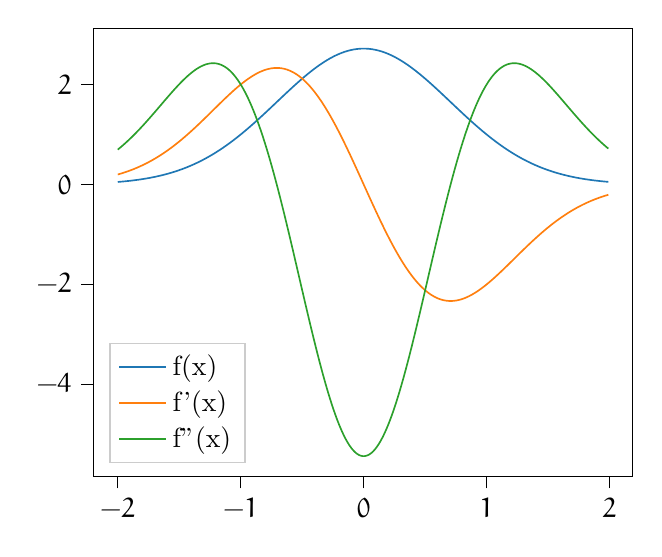
\begin{tikzpicture}

\definecolor{color0}{rgb}{0.12156862745098,0.466666666666667,0.705882352941177}
\definecolor{color1}{rgb}{1,0.498039215686275,0.0549019607843137}
\definecolor{color2}{rgb}{0.172549019607843,0.627450980392157,0.172549019607843}

\begin{axis}[
legend cell align={left},
legend style={
  fill opacity=0.8,
  draw opacity=1,
  text opacity=1,
  at={(0.03,0.03)},
  anchor=south west,
  draw=white!80!black
},
tick align=outside,
tick pos=left,
x grid style={white!69.0196078431373!black},
xmin=-2.1995, xmax=2.1895,
xtick style={color=black},
y grid style={white!69.0196078431373!black},
ymin=-5.84430593118695, ymax=3.1260241027279,
ytick style={color=black}
]
\addplot [semithick, color0]
table {%
-2 0.0497870683678639
-1.99 0.0518137355400945
-1.98 0.0539121181395556
-1.97 0.0560842642753431
-1.96 0.0583322596439408
-1.95 0.06065822734184
-1.94 0.0630643276324908
-1.93 0.0655527576660381
-1.92 0.0681257511503045
-1.91 0.0707855779714885
-1.9 0.0735345437630571
-1.89 0.0763749894213283
-1.88 0.0793092905662537
-1.87 0.0823398569459331
-1.86 0.0854691317834157
-1.85 0.0886995910643704
-1.84 0.0920337427642353
-1.83 0.0954741260134918
-1.82 0.0990233101997463
-1.81 0.10268389400534
-1.8 0.106458504379253
-1.79 0.110349795442121
-1.78 0.11436044732322
-1.77 0.118493164928355
-1.76 0.122750676637611
-1.75 0.127135732932036
-1.74 0.131651104948329
-1.73 0.136299582960754
-1.72 0.141083974789495
-1.71 0.146007104134808
-1.7 0.151071808836371
-1.69 0.156280939057346
-1.68 0.161637355392719
-1.67 0.167143926901625
-1.66 0.172803529063421
-1.65 0.1786190416574
-1.64 0.184593346566117
-1.63 0.190729325502439
-1.62 0.197029857660508
-1.61 0.203497817290952
-1.6 0.210136071200765
-1.59 0.216947476178441
-1.58 0.223934876345025
-1.57 0.231101100431907
-1.56 0.238448958986301
-1.55 0.245981241505487
-1.54 0.253700713501023
-1.53 0.261610113494293
-1.52 0.26971214994486
-1.51 0.278009498113289
-1.5 0.28650479686019
-1.49 0.295200645383424
-1.48 0.304099599895534
-1.47 0.313204170243635
-1.46 0.32251681647411
-1.45 0.332039945344661
-1.44 0.341775906786357
-1.43 0.351726990318523
-1.42 0.361895421419426
-1.41 0.372283357855891
-1.4 0.382892885975113
-1.39 0.393726016962079
-1.38 0.404784683066186
-1.37 0.416070733800749
-1.36 0.427585932119261
-1.35 0.439331950572414
-1.34 0.451310367450007
-1.33 0.463522662912017
-1.32 0.47597021511325
-1.31 0.488654296326095
-1.3 0.501576069066056
-1.29 0.514736582224846
-1.28 0.52813676721593
-1.27 0.541777434137559
-1.26 0.555659267958387
-1.25 0.569782824730924
-1.24 0.584148527838113
-1.23 0.598756664278474
-1.22 0.613607380995284
-1.21 0.628700681255366
-1.2 0.644036421083142
-1.19 0.659614305755633
-1.18 0.675433886364165
-1.17 0.691494556448597
-1.16 0.707795548709892
-1.15 0.724335931806917
-1.14 0.741114607243352
-1.13 0.75813030635062
-1.12 0.77538158737273
-1.11 0.792866832658953
-1.1 0.810584245970189
-1.09 0.828531849904894
-1.08 0.84670748345039
-1.07 0.86510879966531
-1.06 0.883733263498917
-1.05 0.902578149752927
-1.04 0.921640541191413
-1.03 0.940917326804262
-1.02 0.960405200229572
-1.01 0.980100658340256
-0.999999999999999 1
-0.989999999999999 1.02009932499359
-0.979999999999999 1.04039453313647
-0.969999999999999 1.06088132356829
-0.959999999999999 1.0815551942349
-0.949999999999999 1.10241144156333
-0.939999999999999 1.12344516033376
-0.929999999999999 1.14465124375263
-0.919999999999999 1.16602438373056
-0.909999999999999 1.18755907136878
-0.899999999999999 1.20924959765725
-0.889999999999999 1.23109005438778
-0.879999999999999 1.25307433528476
-0.869999999999999 1.27519613735643
-0.859999999999999 1.29744896246868
-0.849999999999999 1.31982611914376
-0.839999999999999 1.34232072458547
-0.829999999999999 1.36492570693246
-0.819999999999999 1.38763380774081
-0.809999999999999 1.41043758469679
-0.799999999999999 1.43332941456034
-0.789999999999999 1.4563014963397
-0.779999999999999 1.47934585469696
-0.769999999999999 1.50245434358429
-0.759999999999999 1.52561865011011
-0.749999999999999 1.54883029863414
-0.739999999999999 1.57208065509
-0.729999999999999 1.59536093153362
-0.719999999999999 1.61866219091532
-0.709999999999999 1.64197535207335
-0.699999999999999 1.66529119494589
-0.689999999999999 1.68860036599858
-0.679999999999999 1.71189338386407
-0.669999999999999 1.73516064518973
-0.659999999999999 1.75839243068945
-0.649999999999999 1.78157891139506
-0.639999999999999 1.80471015510234
-0.629999999999999 1.8277761330067
-0.619999999999999 1.85076672652285
-0.609999999999999 1.87367173428265
-0.599999999999999 1.89648087930495
-0.589999999999999 1.91918381633104
-0.579999999999999 1.9417701393187
-0.569999999999999 1.96422938908794
-0.559999999999999 1.98655106111088
-0.549999999999999 2.00872461343814
-0.539999999999999 2.03073947475375
-0.529999999999999 2.0525850525502
-0.519999999999999 2.07425074141537
-0.509999999999999 2.09572593142225
-0.499999999999999 2.11700001661268
-0.489999999999999 2.1380624035658
-0.479999999999999 2.15890252004167
-0.469999999999999 2.17950982369053
-0.459999999999999 2.19987381081777
-0.449999999999999 2.21998402519458
-0.439999999999999 2.23983006690418
-0.429999999999999 2.25940160121319
-0.419999999999999 2.27868836745778
-0.409999999999999 2.29768018793391
-0.399999999999999 2.31636697678109
-0.389999999999999 2.33473874884891
-0.379999999999999 2.3527856285353
-0.369999999999999 2.370497858586
-0.359999999999999 2.38786580884402
-0.349999999999999 2.40487998493829
-0.339999999999999 2.42153103690064
-0.329999999999999 2.43780976770008
-0.319999999999999 2.45370714168361
-0.309999999999998 2.46921429291272
-0.299999999999998 2.48432253338482
-0.289999999999998 2.49902336112901
-0.279999999999998 2.51330846816559
-0.269999999999998 2.52716974831896
-0.259999999999998 2.54059930487359
-0.249999999999998 2.55358945806293
-0.239999999999998 2.56613275238149
-0.229999999999998 2.57822196371009
-0.219999999999998 2.589850106245
-0.209999999999998 2.60101043922155
-0.199999999999998 2.61169647342312
-0.189999999999998 2.62190197746688
-0.179999999999998 2.63162098385757
-0.169999999999998 2.64084779480119
-0.159999999999998 2.64957698777069
-0.149999999999998 2.657803420816
-0.139999999999998 2.66552223761111
-0.129999999999998 2.67272887223137
-0.119999999999998 2.67941905365426
-0.109999999999998 2.6855888099776
-0.0999999999999983 2.69123447234926
-0.0899999999999983 2.69635267860294
-0.0799999999999983 2.70094037659499
-0.0699999999999983 2.70499482723765
-0.0599999999999983 2.70851360722449
-0.0499999999999983 2.71149461144418
-0.0399999999999983 2.71393605507931
-0.0299999999999983 2.71583647538738
-0.0199999999999982 2.71719473316122
-0.00999999999999823 2.71801001386716
1.77635683940025e-15 2.71828182845905
0.0100000000000016 2.71801001386716
0.0200000000000018 2.71719473316122
0.030000000000002 2.71583647538738
0.0400000000000018 2.71393605507931
0.0500000000000016 2.71149461144417
0.0600000000000018 2.70851360722449
0.0700000000000021 2.70499482723765
0.0800000000000018 2.70094037659499
0.0900000000000016 2.69635267860294
0.100000000000002 2.69123447234926
0.110000000000002 2.6855888099776
0.120000000000002 2.67941905365426
0.130000000000002 2.67272887223137
0.140000000000002 2.66552223761111
0.150000000000002 2.65780342081599
0.160000000000002 2.64957698777069
0.170000000000002 2.64084779480118
0.180000000000002 2.63162098385756
0.190000000000002 2.62190197746688
0.200000000000002 2.61169647342312
0.210000000000002 2.60101043922154
0.220000000000002 2.589850106245
0.230000000000002 2.57822196371008
0.240000000000002 2.56613275238148
0.250000000000002 2.55358945806292
0.260000000000002 2.54059930487358
0.270000000000002 2.52716974831896
0.280000000000002 2.51330846816559
0.290000000000002 2.499023361129
0.300000000000002 2.48432253338481
0.310000000000002 2.46921429291271
0.320000000000002 2.4537071416836
0.330000000000002 2.43780976770007
0.340000000000002 2.42153103690063
0.350000000000002 2.40487998493828
0.360000000000002 2.38786580884401
0.370000000000002 2.370497858586
0.380000000000002 2.35278562853529
0.390000000000002 2.3347387488489
0.400000000000002 2.31636697678109
0.410000000000002 2.2976801879339
0.420000000000002 2.27868836745777
0.430000000000002 2.25940160121319
0.440000000000002 2.23983006690417
0.450000000000002 2.21998402519458
0.460000000000002 2.19987381081776
0.470000000000002 2.17950982369053
0.480000000000002 2.15890252004166
0.490000000000002 2.13806240356579
0.500000000000002 2.11700001661267
0.510000000000002 2.09572593142224
0.520000000000002 2.07425074141536
0.530000000000002 2.0525850525502
0.540000000000002 2.03073947475374
0.550000000000002 2.00872461343813
0.560000000000002 1.98655106111087
0.570000000000002 1.96422938908793
0.580000000000002 1.9417701393187
0.590000000000003 1.91918381633104
0.600000000000002 1.89648087930495
0.610000000000002 1.87367173428264
0.620000000000002 1.85076672652284
0.630000000000003 1.82777613300669
0.640000000000002 1.80471015510233
0.650000000000002 1.78157891139505
0.660000000000002 1.75839243068945
0.670000000000003 1.73516064518972
0.680000000000002 1.71189338386406
0.690000000000002 1.68860036599858
0.700000000000002 1.66529119494588
0.710000000000003 1.64197535207334
0.720000000000002 1.61866219091531
0.730000000000002 1.59536093153361
0.740000000000002 1.57208065508999
0.750000000000003 1.54883029863413
0.760000000000002 1.5256186501101
0.770000000000002 1.50245434358428
0.780000000000002 1.47934585469695
0.790000000000003 1.4563014963397
0.800000000000002 1.43332941456033
0.810000000000002 1.41043758469678
0.820000000000003 1.3876338077408
0.830000000000003 1.36492570693245
0.840000000000003 1.34232072458546
0.850000000000002 1.31982611914375
0.860000000000003 1.29744896246867
0.870000000000003 1.27519613735642
0.880000000000003 1.25307433528475
0.890000000000002 1.23109005438777
0.900000000000003 1.20924959765725
0.910000000000003 1.18755907136877
0.920000000000003 1.16602438373055
0.930000000000002 1.14465124375262
0.940000000000003 1.12344516033375
0.950000000000003 1.10241144156332
0.960000000000003 1.08155519423489
0.970000000000002 1.06088132356828
0.980000000000003 1.04039453313647
0.990000000000003 1.02009932499358
1 0.999999999999995
1.01 0.98010065834025
1.02 0.960405200229565
1.03 0.940917326804255
1.04 0.921640541191407
1.05 0.902578149752921
1.06 0.88373326349891
1.07 0.865108799665303
1.08 0.846707483450383
1.09 0.828531849904888
1.1 0.810584245970182
1.11 0.792866832658946
1.12 0.775381587372724
1.13 0.758130306350614
1.14 0.741114607243346
1.15 0.724335931806911
1.16 0.707795548709886
1.17 0.691494556448592
1.18 0.67543388636416
1.19 0.659614305755627
1.2 0.644036421083137
1.21 0.628700681255361
1.22 0.613607380995278
1.23 0.598756664278469
1.24 0.584148527838108
1.25 0.569782824730919
1.26 0.555659267958383
1.27 0.541777434137553
1.28 0.528136767215925
1.29 0.514736582224841
1.3 0.501576069066052
1.31 0.48865429632609
1.32 0.475970215113246
1.33 0.463522662912013
1.34 0.451310367450003
1.35 0.43933195057241
1.36 0.427585932119257
1.37 0.416070733800745
1.38 0.404784683066182
1.39 0.393726016962075
1.4 0.382892885975109
1.41 0.372283357855888
1.42 0.361895421419422
1.43 0.351726990318519
1.44 0.341775906786354
1.45 0.332039945344658
1.46 0.322516816474107
1.47 0.313204170243631
1.48 0.304099599895531
1.49 0.295200645383421
1.5 0.286504796860187
1.51 0.278009498113286
1.52 0.269712149944857
1.53 0.26161011349429
1.54 0.253700713501021
1.55 0.245981241505484
1.56 0.238448958986298
1.57 0.231101100431904
1.58 0.223934876345022
1.59 0.216947476178439
1.6 0.210136071200763
1.61 0.20349781729095
1.62 0.197029857660506
1.63 0.190729325502436
1.64 0.184593346566115
1.65 0.178619041657398
1.66 0.172803529063419
1.67 0.167143926901623
1.68 0.161637355392717
1.69 0.156280939057344
1.7 0.151071808836369
1.71 0.146007104134806
1.72 0.141083974789494
1.73 0.136299582960753
1.74 0.131651104948328
1.75 0.127135732932034
1.76 0.12275067663761
1.77 0.118493164928353
1.78 0.114360447323219
1.79 0.110349795442119
1.8 0.106458504379252
1.81 0.102683894005338
1.82 0.099023310199745
1.83 0.0954741260134905
1.84 0.0920337427642341
1.85 0.0886995910643693
1.86 0.0854691317834145
1.87 0.0823398569459319
1.88 0.0793092905662527
1.89 0.0763749894213274
1.9 0.0735345437630561
1.91 0.0707855779714875
1.92 0.0681257511503036
1.93 0.0655527576660372
1.94 0.06306432763249
1.95 0.0606582273418391
1.96 0.0583322596439399
1.97 0.0560842642753424
1.98 0.0539121181395549
1.99 0.0518137355400937
};
\addlegendentry{f(x)}
\addplot [semithick, color1]
table {%
-2 0.199148273471456
-1.99 0.206218667449576
-1.98 0.21349198783264
-1.97 0.220972001244852
-1.96 0.228662457804248
-1.95 0.236567086633176
-1.94 0.244689591214064
-1.93 0.253033644590907
-1.92 0.261602884417169
-1.91 0.270400907851086
-1.9 0.279431266299617
-1.89 0.288697460012621
-1.88 0.298202932529114
-1.87 0.30795106497779
-1.86 0.317945170234306
-1.85 0.328188486938171
-1.84 0.338684173372386
-1.83 0.34943530120938
-1.82 0.360444849127076
-1.81 0.37171569629933
-1.8 0.38325061576531
-1.79 0.395052267682791
-1.78 0.407123192470663
-1.77 0.419465803846375
-1.76 0.432082381764392
-1.75 0.444975065262125
-1.74 0.458145845220185
-1.73 0.47159655704421
-1.72 0.485328873275864
-1.71 0.499344296141042
-1.7 0.513644150043661
-1.69 0.528229574013829
-1.68 0.543101514119535
-1.67 0.558260715851427
-1.66 0.573707716490559
-1.65 0.58944283746942
-1.64 0.605466176736863
-1.63 0.62177760113795
-1.62 0.638376738820047
-1.61 0.655262971676864
-1.6 0.672435427842448
-1.59 0.689892974247443
-1.58 0.707634209250279
-1.57 0.725657455356187
-1.56 0.743960752037258
-1.55 0.762541848667008
-1.54 0.781398197583152
-1.53 0.800526947292536
-1.52 0.819924935832374
-1.51 0.839588684302134
-1.5 0.859514390580571
-1.49 0.879697923242603
-1.48 0.900134815690781
-1.47 0.920820260516286
-1.46 0.941749104104402
-1.45 0.962915841499517
-1.44 0.984314611544708
-1.43 1.00593919231098
-1.42 1.02778299683117
-1.41 1.04983906915361
-1.4 1.07210008073031
-1.39 1.09455832715458
-1.38 1.11720572526267
-1.37 1.14003381061405
-1.36 1.16303373536439
-1.35 1.18619626654552
-1.34 1.20951178476602
-1.33 1.23297028334597
-1.32 1.25656136789898
-1.31 1.28027425637437
-1.3 1.30409777957175
-1.29 1.3280203821401
-1.28 1.35203012407278
-1.27 1.3761146827094
-1.26 1.40026135525514
-1.25 1.42445706182731
-1.24 1.44868834903852
-1.23 1.47294139412505
-1.22 1.49720200962849
-1.21 1.52145564863798
-1.2 1.54568741059954
-1.19 1.56988204769841
-1.18 1.59402397181943
-1.17 1.61809726208972
-1.16 1.64208567300695
-1.15 1.66597264315591
-1.14 1.68974130451484
-1.13 1.7133744923524
-1.12 1.73685475571491
-1.11 1.76016436850287
-1.1 1.78328534113441
-1.09 1.80619943279267
-1.08 1.82888816425284
-1.07 1.85133283128376
-1.06 1.8735145186177
-1.05 1.89541411448115
-1.04 1.91701232567814
-1.03 1.93828969321678
-1.02 1.95922660846832
-1.01 1.97980332984732
-0.999999999999999 2
-0.989999999999999 2.01979666348731
-0.979999999999999 2.03917328494749
-0.969999999999999 2.05810976772248
-0.959999999999999 2.076585972931
-0.949999999999999 2.09458173897032
-0.939999999999999 2.11207690142747
-0.929999999999999 2.12905131337988
-0.919999999999999 2.14548486606423
-0.909999999999999 2.16135750989117
-0.899999999999999 2.17664927578305
-0.889999999999999 2.19134029681024
-0.879999999999999 2.20541083010118
-0.869999999999999 2.21884127900018
-0.859999999999999 2.23161221544613
-0.849999999999999 2.24370440254439
-0.839999999999999 2.25509881730358
-0.829999999999999 2.26577667350787
-0.819999999999999 2.27571944469493
-0.809999999999999 2.28490888720879
-0.799999999999999 2.29332706329655
-0.789999999999999 2.30095636421673
-0.779999999999999 2.30777953332726
-0.769999999999999 2.3137796891198
-0.759999999999999 2.31894034816736
-0.749999999999999 2.3232454479512
-0.739999999999999 2.3266793695332
-0.729999999999999 2.32922696003908
-0.719999999999999 2.33087355491806
-0.709999999999999 2.33160499994415
-0.699999999999999 2.33140767292424
-0.689999999999999 2.33026850507804
-0.679999999999999 2.32817500205513
-0.669999999999999 2.32511526455423
-0.659999999999999 2.32107800851008
-0.649999999999999 2.31605258481357
-0.639999999999999 2.31002899853099
-0.629999999999999 2.30299792758843
-0.619999999999999 2.29495074088833
-0.609999999999999 2.28587951582482
-0.599999999999999 2.27577705516594
-0.589999999999999 2.26463690327063
-0.579999999999999 2.25245336160969
-0.569999999999999 2.23922150356025
-0.559999999999999 2.22493718844418
-0.549999999999999 2.20959707478195
-0.539999999999999 2.19319863273404
-0.529999999999999 2.17574015570321
-0.519999999999999 2.15722077107198
-0.509999999999999 2.13764045005069
-0.499999999999999 2.11700001661267
-0.489999999999999 2.09530115549447
-0.479999999999999 2.07254641924
-0.469999999999999 2.0487392342691
-0.459999999999999 2.02388390595234
-0.449999999999999 1.99798562267512
-0.439999999999999 1.97105045887567
-0.429999999999999 1.94308537704334
-0.419999999999999 1.91409822866453
-0.409999999999999 1.8840977541058
-0.399999999999999 1.85309358142487
-0.389999999999999 1.82109622410214
-0.379999999999999 1.78811707768682
-0.369999999999999 1.75416841535364
-0.359999999999999 1.71926338236769
-0.349999999999999 1.6834159894568
-0.339999999999999 1.64664110509243
-0.329999999999999 1.60895444668204
-0.319999999999999 1.5703725706775
-0.309999999999998 1.53091286160588
-0.299999999999998 1.49059352003088
-0.289999999999998 1.44943354945482
-0.279999999999998 1.40745274217272
-0.269999999999998 1.36467166409223
-0.259999999999998 1.32111163853426
-0.249999999999998 1.27679472903146
-0.239999999999998 1.23174372114311
-0.229999999999998 1.18598210330663
-0.219999999999998 1.13953404674779
-0.209999999999998 1.09242438447304
-0.199999999999998 1.04467858936924
-0.189999999999998 0.996322751437407
-0.179999999999998 0.947383554188716
-0.169999999999998 0.897888250232395
-0.159999999999998 0.847864636086612
-0.149999999999998 0.79734102624479
-0.139999999999998 0.746346226531103
-0.129999999999998 0.694909506780147
-0.119999999999998 0.643060572877013
-0.109999999999998 0.590829538195063
-0.0999999999999983 0.538246894469844
-0.0899999999999983 0.48534348214852
-0.0799999999999983 0.432150460255189
-0.0699999999999983 0.378699275813262
-0.0599999999999983 0.32502163286693
-0.0499999999999983 0.271149461144408
-0.0399999999999983 0.217114884406336
-0.0299999999999983 0.162950188523233
-0.0199999999999982 0.108687789326439
-0.00999999999999823 0.0543602002773335
1.77635683940025e-15 -9.65727703480129e-15
0.0100000000000016 -0.0543602002773516
0.0200000000000018 -0.108687789326458
0.030000000000002 -0.162950188523254
0.0400000000000018 -0.217114884406355
0.0500000000000016 -0.271149461144426
0.0600000000000018 -0.325021632866949
0.0700000000000021 -0.378699275813282
0.0800000000000018 -0.432150460255208
0.0900000000000016 -0.485343482148538
0.100000000000002 -0.538246894469862
0.110000000000002 -0.590829538195083
0.120000000000002 -0.643060572877032
0.130000000000002 -0.694909506780165
0.140000000000002 -0.746346226531121
0.150000000000002 -0.79734102624481
0.160000000000002 -0.84786463608663
0.170000000000002 -0.897888250232411
0.180000000000002 -0.947383554188733
0.190000000000002 -0.996322751437425
0.200000000000002 -1.04467858936926
0.210000000000002 -1.09242438447306
0.220000000000002 -1.13953404674781
0.230000000000002 -1.18598210330665
0.240000000000002 -1.23174372114312
0.250000000000002 -1.27679472903147
0.260000000000002 -1.32111163853427
0.270000000000002 -1.36467166409225
0.280000000000002 -1.40745274217274
0.290000000000002 -1.44943354945483
0.300000000000002 -1.4905935200309
0.310000000000002 -1.53091286160589
0.320000000000002 -1.57037257067752
0.330000000000002 -1.60895444668206
0.340000000000002 -1.64664110509244
0.350000000000002 -1.68341598945681
0.360000000000002 -1.7192633823677
0.370000000000002 -1.75416841535365
0.380000000000002 -1.78811707768683
0.390000000000002 -1.82109622410215
0.400000000000002 -1.85309358142488
0.410000000000002 -1.88409775410581
0.420000000000002 -1.91409822866454
0.430000000000002 -1.94308537704335
0.440000000000002 -1.97105045887568
0.450000000000002 -1.99798562267513
0.460000000000002 -2.02388390595235
0.470000000000002 -2.0487392342691
0.480000000000002 -2.07254641924
0.490000000000002 -2.09530115549448
0.500000000000002 -2.11700001661268
0.510000000000002 -2.13764045005069
0.520000000000002 -2.15722077107199
0.530000000000002 -2.17574015570322
0.540000000000002 -2.19319863273405
0.550000000000002 -2.20959707478196
0.560000000000002 -2.22493718844418
0.570000000000002 -2.23922150356025
0.580000000000002 -2.2524533616097
0.590000000000003 -2.26463690327063
0.600000000000002 -2.27577705516594
0.610000000000002 -2.28587951582483
0.620000000000002 -2.29495074088833
0.630000000000003 -2.30299792758844
0.640000000000002 -2.31002899853099
0.650000000000002 -2.31605258481358
0.660000000000002 -2.32107800851008
0.670000000000003 -2.32511526455423
0.680000000000002 -2.32817500205513
0.690000000000002 -2.33026850507804
0.700000000000002 -2.33140767292424
0.710000000000003 -2.33160499994415
0.720000000000002 -2.33087355491806
0.730000000000002 -2.32922696003908
0.740000000000002 -2.3266793695332
0.750000000000003 -2.3232454479512
0.760000000000002 -2.31894034816736
0.770000000000002 -2.3137796891198
0.780000000000002 -2.30777953332726
0.790000000000003 -2.30095636421673
0.800000000000002 -2.29332706329654
0.810000000000002 -2.28490888720879
0.820000000000003 -2.27571944469492
0.830000000000003 -2.26577667350787
0.840000000000003 -2.25509881730358
0.850000000000002 -2.24370440254439
0.860000000000003 -2.23161221544613
0.870000000000003 -2.21884127900018
0.880000000000003 -2.20541083010117
0.890000000000002 -2.19134029681023
0.900000000000003 -2.17664927578305
0.910000000000003 -2.16135750989117
0.920000000000003 -2.14548486606422
0.930000000000002 -2.12905131337988
0.940000000000003 -2.11207690142746
0.950000000000003 -2.09458173897031
0.960000000000003 -2.076585972931
0.970000000000002 -2.05810976772247
0.980000000000003 -2.03917328494748
0.990000000000003 -2.0197966634873
1 -1.99999999999999
1.01 -1.97980332984731
1.02 -1.95922660846832
1.03 -1.93828969321677
1.04 -1.91701232567813
1.05 -1.89541411448114
1.06 -1.87351451861769
1.07 -1.85133283128375
1.08 -1.82888816425283
1.09 -1.80619943279266
1.1 -1.78328534113441
1.11 -1.76016436850287
1.12 -1.7368547557149
1.13 -1.71337449235239
1.14 -1.68974130451483
1.15 -1.6659726431559
1.16 -1.64208567300694
1.17 -1.61809726208971
1.18 -1.59402397181942
1.19 -1.5698820476984
1.2 -1.54568741059953
1.21 -1.52145564863798
1.22 -1.49720200962848
1.23 -1.47294139412504
1.24 -1.44868834903851
1.25 -1.4244570618273
1.26 -1.40026135525513
1.27 -1.37611468270939
1.28 -1.35203012407277
1.29 -1.32802038214009
1.3 -1.30409777957174
1.31 -1.28027425637436
1.32 -1.25656136789897
1.33 -1.23297028334596
1.34 -1.20951178476601
1.35 -1.18619626654551
1.36 -1.16303373536438
1.37 -1.14003381061404
1.38 -1.11720572526267
1.39 -1.09455832715457
1.4 -1.07210008073031
1.41 -1.04983906915361
1.42 -1.02778299683116
1.43 -1.00593919231097
1.44 -0.984314611544701
1.45 -0.96291584149951
1.46 -0.941749104104394
1.47 -0.920820260516278
1.48 -0.900134815690774
1.49 -0.879697923242596
1.5 -0.859514390580564
1.51 -0.839588684302126
1.52 -0.819924935832368
1.53 -0.800526947292529
1.54 -0.781398197583145
1.55 -0.762541848667001
1.56 -0.743960752037252
1.57 -0.725657455356181
1.58 -0.707634209250272
1.59 -0.689892974247436
1.6 -0.672435427842442
1.61 -0.655262971676859
1.62 -0.638376738820041
1.63 -0.621777601137944
1.64 -0.605466176736858
1.65 -0.589442837469415
1.66 -0.573707716490553
1.67 -0.558260715851421
1.68 -0.54310151411953
1.69 -0.528229574013824
1.7 -0.513644150043656
1.71 -0.499344296141036
1.72 -0.485328873275859
1.73 -0.471596557044206
1.74 -0.458145845220181
1.75 -0.44497506526212
1.76 -0.432082381764388
1.77 -0.419465803846371
1.78 -0.407123192470659
1.79 -0.395052267682787
1.8 -0.383250615765306
1.81 -0.371715696299326
1.82 -0.360444849127073
1.83 -0.349435301209376
1.84 -0.338684173372382
1.85 -0.328188486938167
1.86 -0.317945170234303
1.87 -0.307951064977786
1.88 -0.298202932529111
1.89 -0.288697460012618
1.9 -0.279431266299614
1.91 -0.270400907851083
1.92 -0.261602884417166
1.93 -0.253033644590904
1.94 -0.244689591214062
1.95 -0.236567086633173
1.96 -0.228662457804245
1.97 -0.220972001244849
1.98 -0.213491987832638
1.99 -0.206218667449573
};
\addlegendentry{f'(x)}
\addplot [semithick, color2]
table {%
-2 0.697018957150095
-1.99 0.717122825369124
-1.98 0.737604035538144
-1.97 0.75846115635403
-1.96 0.77969231530477
-1.95 0.801295183185707
-1.94 0.823266958645588
-1.93 0.845604352788825
-1.92 0.868303573861321
-1.91 0.891360312048171
-1.9 0.91476972441243
-1.89 0.938526420005051
-1.88 0.962624445176961
-1.87 0.987057269125067
-1.86 1.01181776970479
-1.85 1.03689821954249
-1.84 1.06229027248191
-1.83 1.08798495039935
-1.82 1.11397263042307
-1.81 1.14024303259289
-1.8 1.16678520799661
-1.79 1.19358752742015
-1.78 1.22063767054912
-1.77 1.24792261575946
-1.76 1.27542863053544
-1.75 1.30314126255337
-1.74 1.33104533146959
-1.73 1.35912492145146
-1.72 1.38736337448998
-1.71 1.41574328453275
-1.7 1.44424649247571
-1.69 1.47285408205205
-1.68 1.5015463766562
-1.67 1.53030293714052
-1.66 1.55910256062181
-1.65 1.58792328033429
-1.64 1.61674236656468
-1.63 1.64553632870484
-1.62 1.67428091845593
-1.61 1.7029511342176
-1.6 1.7315212266943
-1.59 1.75996470574999
-1.58 1.78825434854083
-1.57 1.81636220895461
-1.56 1.84425962838364
-1.55 1.87191724785675
-1.54 1.89930502155406
-1.53 1.92639223172657
-1.52 1.9531475050407
-1.51 1.97953883036586
-1.5 2.00553357802133
-1.49 2.03109852049611
-1.48 2.05619985465364
-1.47 2.08080322543061
-1.46 2.10487375103663
-1.45 2.12837604965928
-1.44 2.15127426767604
-1.43 2.17353210937234
-1.42 2.19511286816167
-1.41 2.21597945930141
-1.4 2.23609445409466
-1.39 2.25542011556557
-1.38 2.27391843559261
-1.37 2.291551173481
-1.36 2.30827989595262
-1.35 2.32406601852807
-1.34 2.33887084827291
-1.33 2.35265562787623
-1.32 2.36538158102681
-1.31 2.37700995904865
-1.3 2.38750208875443
-1.29 2.39681942147177
-1.28 2.40492358319446
-1.27 2.41177642580675
-1.26 2.41734007932617
-1.25 2.42157700510642
-1.24 2.4244500499393
-1.23 2.42592250099066
-1.22 2.42595814150295
-1.21 2.42452130719319
-1.2 2.42157694327261
-1.19 2.41709066201094
-1.18 2.41102880076552
-1.17 2.40335848039274
-1.16 2.39404766395633
-1.15 2.38306521564475
-1.14 2.37038095980713
-1.13 2.35596574001518
-1.12 2.33979147805594
-1.11 2.32183123275847
-1.1 2.30205925855533
-1.09 2.28045106367823
-1.08 2.25698346788535
-1.07 2.23163465961663
-1.06 2.20438425247169
-1.05 2.17521334090455
-1.04 2.1441045550277
-1.03 2.11104211441804
-1.02 2.07601188081624
-1.01 2.03900140961106
-0.999999999999999 2
-0.989999999999999 1.95899874371769
-0.979999999999999 1.91599057222412
-0.969999999999999 1.87097030224502
-0.959999999999999 1.82393467955773
-0.949999999999999 1.77488242091695
-0.939999999999999 1.72381425401611
-0.929999999999999 1.67073295538133
-0.919999999999999 1.61564338609706
-0.909999999999999 1.55855252526438
-0.899999999999999 1.49946950109499
-0.889999999999999 1.43840561954667
-0.879999999999999 1.37537439040854
-0.869999999999999 1.31039155074746
-0.859999999999999 1.24347508562998
-0.849999999999999 1.17464524603794
-0.839999999999999 1.10392456389908
-0.829999999999999 1.03133786415815
-0.819999999999999 0.956912273818054
-0.809999999999999 0.880677227884665
-0.799999999999999 0.802664472153782
-0.789999999999999 0.722908062783019
-0.779999999999999 0.641444362596593
-0.769999999999999 0.558312034075912
-0.759999999999999 0.473552028994167
-0.749999999999999 0.387207574658524
-0.739999999999999 0.299324156729126
-0.729999999999999 0.209949498589814
-0.719999999999999 0.119133537251357
-0.709999999999999 0.026928395773992
-0.699999999999999 -0.0666116477978463
-0.689999999999999 -0.161430194989475
-0.679999999999999 -0.257468764933167
-0.669999999999999 -0.354666835876791
-0.659999999999999 -0.452961890145615
-0.649999999999999 -0.55228946253248
-0.639999999999999 -0.652583192085016
-0.629999999999999 -0.753774877251973
-0.619999999999999 -0.855794534344177
-0.609999999999999 -0.958570459259014
-0.599999999999999 -1.06202929241079
-0.589999999999999 -1.16609608680275
-0.579999999999999 -1.27069437917017
-0.569999999999999 -1.3757462641172
-0.559999999999999 -1.48117247116428
-0.549999999999999 -1.58689244461614
-0.539999999999999 -1.69282442615474
-0.529999999999999 -1.79888554005501
-0.519999999999999 -1.90499188091589
-0.509999999999999 -2.0110586037928
-0.499999999999999 -2.11700001661269
-0.489999999999999 -2.22272967474701
-0.479999999999999 -2.32816047761295
-0.469999999999999 -2.43320476716812
-0.459999999999999 -2.53777442815939
-0.449999999999999 -2.64178098998156
-0.439999999999999 -2.74513572999777
-0.429999999999999 -2.84774977816912
-0.419999999999999 -2.94953422283736
-0.409999999999999 -3.05040021750106
-0.399999999999999 -3.1502590884223
-0.389999999999999 -3.24902244289815
-0.379999999999999 -3.34660227802862
-0.369999999999999 -3.44291108981032
-0.359999999999999 -3.53786198238331
-0.349999999999999 -3.63136877725683
-0.339999999999999 -3.72334612233843
-0.329999999999999 -3.81370960059001
-0.319999999999999 -3.90237583813362
-0.309999999999998 -3.9892626116298
-0.299999999999998 -4.07428895475111
-0.289999999999998 -4.15737526357423
-0.279999999999998 -4.23844340071446
-0.269999999999998 -4.31741679802813
-0.259999999999998 -4.39422055770936
-0.249999999999998 -4.46878155161013
-0.239999999999998 -4.54102851861429
-0.229999999999998 -4.61089215989913
-0.219999999999998 -4.67830523192098
-0.209999999999998 -4.74320263696442
-0.199999999999998 -4.80552151109855
-0.189999999999998 -4.86520130938755
-0.179999999999998 -4.9221838882072
-0.169999999999998 -4.97641358452336
-0.159999999999998 -5.02783729199366
-0.149999999999998 -5.07640453375856
-0.139999999999998 -5.12206753179352
-0.129999999999998 -5.1647812726999
-0.119999999999998 -5.20450356981804
-0.109999999999998 -5.24119512155229
-0.0999999999999983 -5.27481956580456
-0.0899999999999983 -5.30534353041915
-0.0799999999999983 -5.33273667954915
-0.0699999999999983 -5.35697175586145
-0.0599999999999983 -5.37802461850495
-0.0499999999999983 -5.39587427677391
-0.0399999999999983 -5.41050291940612
-0.0299999999999983 -5.42189593946336
-0.0199999999999982 -5.43004195474937
-0.00999999999999823 -5.43493282372876
1.77635683940025e-15 -5.43656365691809
0.0100000000000016 -5.43493282372876
0.0200000000000018 -5.43004195474937
0.030000000000002 -5.42189593946335
0.0400000000000018 -5.41050291940612
0.0500000000000016 -5.3958742767739
0.0600000000000018 -5.37802461850495
0.0700000000000021 -5.35697175586144
0.0800000000000018 -5.33273667954914
0.0900000000000016 -5.30534353041914
0.100000000000002 -5.27481956580455
0.110000000000002 -5.24119512155228
0.120000000000002 -5.20450356981802
0.130000000000002 -5.16478127269989
0.140000000000002 -5.1220675317935
0.150000000000002 -5.07640453375854
0.160000000000002 -5.02783729199365
0.170000000000002 -4.97641358452334
0.180000000000002 -4.92218388820718
0.190000000000002 -4.86520130938753
0.200000000000002 -4.80552151109852
0.210000000000002 -4.7432026369644
0.220000000000002 -4.67830523192095
0.230000000000002 -4.6108921598991
0.240000000000002 -4.54102851861426
0.250000000000002 -4.46878155161011
0.260000000000002 -4.39422055770933
0.270000000000002 -4.3174167980281
0.280000000000002 -4.23844340071443
0.290000000000002 -4.1573752635742
0.300000000000002 -4.07428895475108
0.310000000000002 -3.98926261162976
0.320000000000002 -3.90237583813359
0.330000000000002 -3.81370960058998
0.340000000000002 -3.7233461223384
0.350000000000002 -3.63136877725679
0.360000000000002 -3.53786198238328
0.370000000000002 -3.44291108981029
0.380000000000002 -3.34660227802859
0.390000000000002 -3.24902244289811
0.400000000000002 -3.15025908842226
0.410000000000002 -3.05040021750103
0.420000000000002 -2.94953422283733
0.430000000000002 -2.84774977816908
0.440000000000002 -2.74513572999774
0.450000000000002 -2.64178098998153
0.460000000000002 -2.53777442815936
0.470000000000002 -2.43320476716808
0.480000000000002 -2.32816047761291
0.490000000000002 -2.22272967474698
0.500000000000002 -2.11700001661265
0.510000000000002 -2.01105860379276
0.520000000000002 -1.90499188091585
0.530000000000002 -1.79888554005497
0.540000000000002 -1.6928244261547
0.550000000000002 -1.5868924446161
0.560000000000002 -1.48117247116424
0.570000000000002 -1.37574626411717
0.580000000000002 -1.27069437917013
0.590000000000003 -1.16609608680271
0.600000000000002 -1.06202929241075
0.610000000000002 -0.958570459258979
0.620000000000002 -0.855794534344141
0.630000000000003 -0.753774877251935
0.640000000000002 -0.65258319208498
0.650000000000002 -0.552289462532447
0.660000000000002 -0.45296189014558
0.670000000000003 -0.354666835876754
0.680000000000002 -0.257468764933133
0.690000000000002 -0.161430194989444
0.700000000000002 -0.0666116477978127
0.710000000000003 0.0269283957740275
0.720000000000002 0.11913353725139
0.730000000000002 0.209949498589844
0.740000000000002 0.299324156729158
0.750000000000003 0.387207574658556
0.760000000000002 0.473552028994197
0.770000000000002 0.55831203407594
0.780000000000002 0.641444362596622
0.790000000000003 0.72290806278305
0.800000000000002 0.80266447215381
0.810000000000002 0.88067722788469
0.820000000000003 0.95691227381808
0.830000000000003 1.03133786415818
0.840000000000003 1.1039245638991
0.850000000000002 1.17464524603796
0.860000000000003 1.24347508563
0.870000000000003 1.31039155074748
0.880000000000003 1.37537439040857
0.890000000000002 1.43840561954669
0.900000000000003 1.49946950109501
0.910000000000003 1.5585525252644
0.920000000000003 1.61564338609708
0.930000000000002 1.67073295538134
0.940000000000003 1.72381425401613
0.950000000000003 1.77488242091697
0.960000000000003 1.82393467955774
0.970000000000002 1.87097030224504
0.980000000000003 1.91599057222414
0.990000000000003 1.9589987437177
1 2.00000000000001
1.01 2.03900140961108
1.02 2.07601188081625
1.03 2.11104211441805
1.04 2.14410455502771
1.05 2.17521334090456
1.06 2.2043842524717
1.07 2.23163465961664
1.08 2.25698346788536
1.09 2.28045106367823
1.1 2.30205925855534
1.11 2.32183123275848
1.12 2.33979147805595
1.13 2.35596574001518
1.14 2.37038095980714
1.15 2.38306521564476
1.16 2.39404766395634
1.17 2.40335848039274
1.18 2.41102880076552
1.19 2.41709066201094
1.2 2.42157694327261
1.21 2.42452130719319
1.22 2.42595814150295
1.23 2.42592250099066
1.24 2.4244500499393
1.25 2.42157700510642
1.26 2.41734007932616
1.27 2.41177642580675
1.28 2.40492358319445
1.29 2.39681942147177
1.3 2.38750208875442
1.31 2.37700995904865
1.32 2.3653815810268
1.33 2.35265562787623
1.34 2.33887084827291
1.35 2.32406601852806
1.36 2.30827989595261
1.37 2.291551173481
1.38 2.2739184355926
1.39 2.25542011556556
1.4 2.23609445409465
1.41 2.2159794593014
1.42 2.19511286816166
1.43 2.17353210937233
1.44 2.15127426767604
1.45 2.12837604965927
1.46 2.10487375103662
1.47 2.0808032254306
1.48 2.05619985465363
1.49 2.0310985204961
1.5 2.00553357802132
1.51 1.97953883036585
1.52 1.95314750504069
1.53 1.92639223172656
1.54 1.89930502155405
1.55 1.87191724785674
1.56 1.84425962838363
1.57 1.8163622089546
1.58 1.78825434854082
1.59 1.75996470574997
1.6 1.73152122669429
1.61 1.70295113421759
1.62 1.67428091845592
1.63 1.64553632870483
1.64 1.61674236656467
1.65 1.58792328033428
1.66 1.5591025606218
1.67 1.5303029371405
1.68 1.50154637665619
1.69 1.47285408205204
1.7 1.4442464924757
1.71 1.41574328453274
1.72 1.38736337448997
1.73 1.35912492145145
1.74 1.33104533146958
1.75 1.30314126255335
1.76 1.27542863053543
1.77 1.24792261575945
1.78 1.22063767054911
1.79 1.19358752742014
1.8 1.1667852079966
1.81 1.14024303259289
1.82 1.11397263042306
1.83 1.08798495039934
1.84 1.0622902724819
1.85 1.03689821954248
1.86 1.01181776970478
1.87 0.987057269125058
1.88 0.962624445176953
1.89 0.938526420005043
1.9 0.914769724412422
1.91 0.891360312048163
1.92 0.868303573861313
1.93 0.845604352788817
1.94 0.82326695864558
1.95 0.801295183185698
1.96 0.779692315304762
1.97 0.758461156354023
1.98 0.737604035538137
1.99 0.717122825369116
};
\addlegendentry{f"(x)}
\end{axis}

\end{tikzpicture}

\end{center}
\caption{\label{fig:fgh}The simple function and its derivatives}
\end{figure}

\section{Estimation and simple simulation}

\begin{flushright}
See \lstinline$02estimation.py$ in Section~\ref{sec:02estimation}
\end{flushright}

We consider a case study involving a transportation mode choice model,
using revealed preference data collected in Switzerland in 2009 and
2010 (see~\cite{AtaGlerBier2012_DISP}).
The model is a nested logit model with 3 alternatives: \emph{public
  transportation}, \emph{car} and \emph{slow modes}. The utility functions are defined as:
\begin{lstlisting}[style=nonumbers,backgroundcolor=]
V_PT = BETA_TIME_FULLTIME * TimePT_scaled * fulltime +
       BETA_TIME_OTHER * TimePT_scaled * notfulltime +
       BETA_COST * MarginalCostPT_scaled
V_CAR = ASC_CAR +
        BETA_TIME_FULLTIME * TimeCar_scaled * fulltime +
        BETA_TIME_OTHER * TimeCar_scaled * notfulltime +
        BETA_COST * CostCarCHF_scaled
V_SM = ASC_SM +
       BETA_DIST_MALE * distance_km_scaled * male  +
       BETA_DIST_FEMALE * distance_km_scaled * female +
       BETA_DIST_UNREPORTED * distance_km_scaled * unreportedGender
\end{lstlisting}
where
\lstinline@ASC_CAR@,
\lstinline@ASC_SM@,
\lstinline@BETA_TIME_FULLTIME@,
\lstinline@BETA_TIME_OTHER@,
\lstinline@BETA_DIST_MALE@,
\lstinline@BETA_DIST_FEMALE@,
\lstinline@BETA_DIST_UNREPORTED@,
\lstinline@BETA_COST@,
are parameters to be estimated,
\lstinline@TimePT_scale@,
\lstinline@MarginalCostPT_scaled@,
\lstinline@TimeCar_scale@,
\lstinline@CostCarCHF_scale@,
\lstinline@distance_km_scale@
are attributes and
\lstinline@fulltime@,
\lstinline@notfulltime@,
\lstinline@male@,
\lstinline@female@,
\lstinline@unreportedGender@ are socio-economic characteristics.
The two alternatives ``public transportation'' and ``slow modes'' are
grouped into a nest.
The complete specification is available in the file
\lstinline$scenarios.py$ reported in
Section~\ref{sec:scenarios}. We refer the reader to
\citeasnoun{Bier18} for an introduction to the syntax.

The parameters are estimated using PandasBiogeme. Their values are
reported in Table~\ref{tab:estimatedParameters}. Note that it is
recommended to perform bootstrapping on the estimation results, in
order to be able to derive confidence intervals for simulated
quantities:
\begin{lstlisting}[style=nonumbers]
results = biogeme.estimate(bootstrap=100)
\end{lstlisting}

\begin{table}[htb]
  \begin{tabular}{l}
\begin{tabular}{rlr@{.}lr@{.}lr@{.}lr@{.}l}
         &                       &   \multicolumn{2}{l}{}    & \multicolumn{2}{l}{Robust}  &     \multicolumn{4}{l}{}   \\
Parameter &                       &   \multicolumn{2}{l}{Coeff.}      & \multicolumn{2}{l}{Asympt.}  &     \multicolumn{4}{l}{}   \\
number &  Description                     &   \multicolumn{2}{l}{estimate}      & \multicolumn{2}{l}{std. error}  &   \multicolumn{2}{l}{$t$-stat}  &   \multicolumn{2}{l}{$p$-value}   \\

\hline

1 & \lstinline@ASC_CAR@ & 0&261 & 0&100 & 2&61 & 0&01\\
2 & \lstinline@ASC_SM@ & 0&0591 & 0&217 & 0&273 & 0&785\\
3 & \lstinline@BETA_COST@ & -0&716 & 0&138 & -5&18 & 0&00\\
4 & \lstinline@BETA_DIST_FEMALE@ & -0&831 & 0&193 & -4&31 & 0&00\\
5 & \lstinline@BETA_DIST_MALE@ & -0&686 & 0&161 & -4&27 & 0&00\\
6 & \lstinline@BETA_DIST_UNREPORTED@ & -0&703 & 0&196 & -3&58 & 0&000344\\
7 & \lstinline@BETA_TIME_FULLTIME@ & -1&60 & 0&333 & -4&80 & 0&00\\
8 & \lstinline@BETA_TIME_OTHER@ & -0&577 & 0&296 & -1&95 & 0&0515\\
9 & \lstinline@NEST_NOCAR@ & 1&53 & 0&306 & 1&73\footnotemark[1] & 0&08\\

\hline
\end{tabular}
\\
\begin{tabular}{rcl}
\multicolumn{3}{l}{\bf Summary statistics}\\
\multicolumn{3}{l}{ Number of observations = $1906$} \\
\multicolumn{3}{l}{ Number of excluded observations = $359$} \\
\multicolumn{3}{l}{ Number of estimated  parameters = $9$} \\
 $\mathcal{L}(\beta_0)$ &=&  $-2093.955$ \\
 $\mathcal{L}(\hat{\beta})$ &=& $-1298.498 $  \\
 $-2[\mathcal{L}(\beta_0) -\mathcal{L}(\hat{\beta})]$ &=& $1590.913$ \\
AIC &=& $2614.997$\\
BIC &=& $2664.971$\\
\end{tabular}
  \end{tabular}
\tablefootnote{$t$-test against 1}
\caption{\protect\label{tab:estimatedParameters}Nested logit model: estimated parameters}
\end{table}

Once the model has been estimated, and the estimation results stored
in the variable \lstinline@results@, simulation can be performed. We
first use simulation to calculate the contribution of each entry of
the database to the log likelihood function. This is actually useful
to identify possible issues with the calculation of the log
likelihood, or to identify outliers, entries associated with low choice
probability.

\begin{lstlisting}[style=nonumbers]
simulated_choices = logprob.getValue_c(
    betas=results.getBetaValues(),
    database=database,
)
\end{lstlisting}
It returns a vector as long as the number of entries in the database,
containing the log of the choice probability for each entry.
The first three entries are $-0.65047242$,  $-1.43260796$,
$-0.13259356$.

The \lstinline@getValue_c@ function  also offers the option to aggregate the
results, and to return the sum. We can use this feature to verify that
it corresponds to the output of the estimation.

\begin{lstlisting}[style=nonumbers]
loglikelihood = logprob.getValue_c(
    betas=results.getBetaValues(),
    database=database,
    aggregation=True,
)
print(f'Final log likelihood:     {results.data.logLike}')
print(f'Simulated log likelihood: {loglikelihood}')
\end{lstlisting}
We obtain the following results:
\begin{lstlisting}[style=nonumbers]
Final log likelihood:     -1298.4982816177392
Simulated log likelihood: -1298.4982816177394
\end{lstlisting}

The complete code associated with this section 
is available in Appendix~\ref{sec:02estimation}.

\section{Simulation and aggregation}

\begin{flushright}
See \lstinline$03simulation.py$ in Section~\ref{sec:03simulation}
\end{flushright}

Clearly, any valid expression can be simulated on the database. When
several of them must be simulated, it may be useful to use the Biogeme
object to simulate them together. For example, suppose that we want to
calculate the values of the utility function and the choice
probability for each alternative, as well as the normalized weight,
for each entry in the database.

This can be done as introduced in the previous section, using the
\lstinline@getValue_c@ function of each expression. But Biogeme
provides a simulation feature that is more efficient, because it
recycles calculated quantities from one expression to the next. A
typical example is the denominator of the choice probability
formula. It is the same for each alternative. If the
\lstinline@getValue_c@ is used for each expression, the denominator
will be recalculated each time. Therefore, the use of the simulation
feature in Biogeme may save a significant amount of time.

The syntax to perform a simulation of several formulas is the
following:

\begin{lstlisting}[style=nonumbers]
simulate = {
    'weight': normalizedWeight,
    'Utility PT': V_PT,
    'Utility car': V_CAR,
    'Utility SM': V_SM,
    'Prob. PT': prob_PT,
    'Prob. car': prob_CAR,
    'Prob. SM': prob_SM,
}
biogeme = bio.BIOGEME(database, simulate)
biogeme_simulation = biogeme.simulate(results.getBetaValues())
\end{lstlisting}

If we perform a comparison of the calculation time with the
\lstinline@getValue_c@ function and with Biogeme, we obtain:
\begin{lstlisting}[style=nonumbers]
--- Execution time with getValue_c: 0.60 seconds ---
--- Execution time with Biogeme:    0.33 seconds ---
\end{lstlisting}
Note that these results vary from one run to the next. 

\section{Market shares and confidence intervals}

\begin{flushright}
See \lstinline$04market_shares.py$ in Section~\ref{sec:04market_shares}
\end{flushright}

Simulation is necessary to derive useful
indicators from an estimated model. We start by describing how to calculate market shares using
sample enumeration. It is necessary to have a sample of individuals
from the population. For each of them, the value of each of the
variables involved in the model must be known.  Note that it is possible to use the same sample
that was used for estimation, but only if it contains revealed
preferences data. Indeed, the calculation of indicators require real
values for the variables, not values that have been designed and engineered for the
sake of estimating parameters, like in stated preferences data. It is the procedure used in this document.

More formally, consider a choice model $P_n(i|x_n, \C_n)$ providing
the probability that individual $n$ chooses alternative $i$ within the
choice set $\C_n$, given the explanatory variables $x_n$.  In order to
calculate the market shares in the population of size $N$, a sample of
$N_s$ individuals is drawn. As it is rarely possible to draw from the
population with equal sampling probability, it is assumed that
stratified sampling has been used, and that each individual $n$ in the
sample is associated with a weight $w_n$ correcting for sampling
biases. The weights are normalized such that
\begin{equation}
  \label{eq:normalizingWeights}
N_s = \sum_{n=1}^{N_s} w_n.
\end{equation}
An estimator of the market share of alternative $i$ in the population is
\begin{equation}
  \label{eq:marketShare}
W_i = \frac{1}{N_s} \sum_{n=1}^{N_s} w_n P_n(i|x_n, \C_n).
\end{equation}
In practice, the size of the population is rarely known, and the above
quantity is used only in the context of price optimization. In this
case, the factor $N/N_s$ can be omitted.

We calculate \req{eq:marketShare} with
PandasBiogeme by simulating the choice probabilities of each
alternative for each entry in the database, as described in the
previous section.

It generates a Pandas data frame. Each row corresponds to an observation
in the Biogeme database, and each column corresponds to a quantity
requested above.

If bootstrapping has been requested during model estimation, 
it is possible to calculate confidence intervals on these
  quantities, using simulation. First, we obtain the results of the
  bootstrapping: 
\begin{lstlisting}
betas = biogeme.freeBetaNames
b = results.getBetasForSensitivityAnalysis(betas)
\end{lstlisting}
And we calculate 90\% confidence intervals:
\begin{lstlisting}
left, right = biogeme.confidenceIntervals(b, 0.9)
\end{lstlisting}
The two generated Pandas data frames have the same structure as the simulated
values, and contain the left and right bounds of the intervals,
respectively.

We can now calculate the market shares, and the confidence
  intervals. We do it below for the car alternative. See
  Appendix~\ref{sec:04market_shares} for the complete code for the
  other alternatives.

  First, we add a column to the data frames for the
  weighted probabilities
  involved in \req{eq:marketShare}:
\begin{lstlisting}
simulated_values['Weighted prob. car'] = (
    simulated_values['weight'] * simulated_values['Prob. car']
)
\end{lstlisting}
 The market shares as well as the confidence intervals,  are simply
 the mean of these new columns:
\begin{lstlisting}
marketShare_car = simulated_values['Weighted prob. car'].mean()
marketShare_car_left = left['Weighted prob. car'].mean()
marketShare_car_right = right['Weighted prob. car'].mean()
\end{lstlisting}

The output of the Python script is as follows:

\begin{lstlisting}
Market share for car: 65.3% [61.4%, 69.0%]
Market share for PT:  28.1% [24.1%, 32.2%]
Market share for SM:   6.6% [4.0%, 9.5%]
\end{lstlisting}

\section{Revenues}

If the alternative $i$ involves a price variable $p_{in}$, the expected revenue
generated by $i$ is
\begin{equation}
  \label{eq:revenues_pop}
\widehat{R}_i = \frac{N}{N_s} \sum_{n=1}^{N_s} w_n p_{in} P_n(i|x_n, p_{in}, \C_n).
\end{equation}
If $N$ is unknown, it is common to use the expected revenues
generated by the individuals in the sample:
\begin{equation}
  \label{eq:revenues_sample}
R_i = \frac{1}{N_s} \sum_{n=1}^{N_s} w_n p_{in} P_n(i|x_n, p_{in}, \C_n).
\end{equation}

In our example, this is calculated by simulating the following quantities:
\begin{lstlisting}[style=nonumbers]
    simulate = {
        'weight': normalizedWeight,
        'Revenue public transportation':
            prob_PT * MarginalCostScenario,
    }
\end{lstlisting}
Then, the total revenues is obtained using:
\begin{lstlisting}[style=nonumbers]
    revenues_pt = (
        simulated_values['Revenue public transportation']
        * simulated_values['weight']
    ).sum()
\end{lstlisting}

Confidence intervals are obtained in a similar way. The result for the
current price is:
\begin{lstlisting}[style=nonumbers, keywordstyle=\ttfamily]
Total revenues for public transportation (for the sample):
    3018.4 CHF [2458.1 CHF, 3664.3 CHF]
\end{lstlisting}
It is also possible to see how the revenues evolve with the price
factor, as illustrated in Figure~\ref{fig:revenues}. The maximum
revenue among the calculated scenarios is also identified:

\begin{lstlisting}[style=nonumbers]
Largest revenue: 3039.1 obtained with factor 1.2
\end{lstlisting}

\begin{figure}
\begin{center}
% This file was created with tikzplotlib v0.9.15.
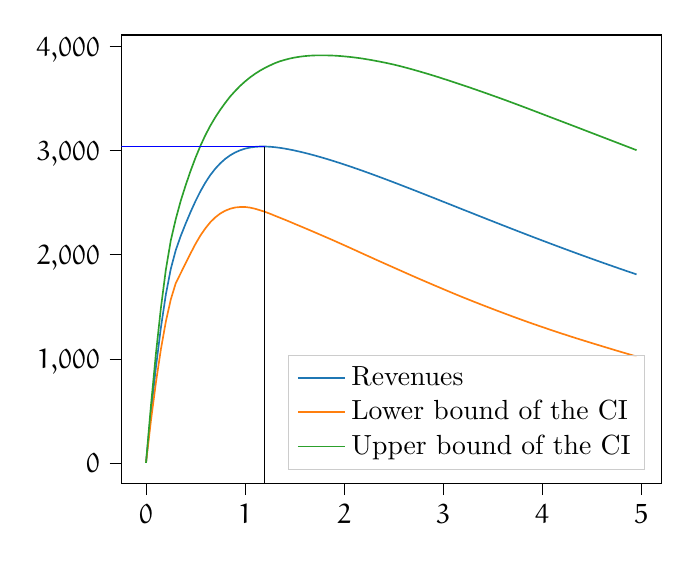
\begin{tikzpicture}

\definecolor{color0}{rgb}{0.12156862745098,0.466666666666667,0.705882352941177}
\definecolor{color1}{rgb}{1,0.498039215686275,0.0549019607843137}
\definecolor{color2}{rgb}{0.172549019607843,0.627450980392157,0.172549019607843}

\begin{axis}[
legend cell align={left},
legend style={
  fill opacity=0.8,
  draw opacity=1,
  text opacity=1,
  at={(0.97,0.03)},
  anchor=south east,
  draw=white!80!black
},
tick align=outside,
tick pos=left,
x grid style={white!69.0196078431373!black},
xmin=-0.2475, xmax=5.1975,
xtick style={color=black},
y grid style={white!69.0196078431373!black},
ymin=-195.738779802373, ymax=4110.51437584982,
ytick style={color=black}
]
\addplot [semithick, color0]
table {%
0 0
0.05 484.135445808616
0.1 917.801179550086
0.15 1297.84909265033
0.2 1616.19111118537
0.25 1863.10445394683
0.3 2042.30470327117
0.35 2178.7603670045
0.4 2298.31369962508
0.45 2410.83935338712
0.5 2515.72806137654
0.55 2610.51966116161
0.6 2693.92637405655
0.65 2765.88202882703
0.7 2827.0104772235
0.75 2878.2198874423
0.8 2920.48774465604
0.85 2954.76809552813
0.9 2981.96009760786
0.95 3002.90179931357
1 3018.37134988233
1.05 3029.08910519688
1.1 3035.71772894662
1.15 3038.86004313851
1.2 3039.05593885971
1.25 3036.77947626918
1.3 3032.43786275747
1.35 3026.37301726789
1.4 3018.86594192792
1.45 3010.14309881215
1.5 3000.38434801883
1.55 2989.73100841497
1.6 2978.29376240798
1.65 2966.15975320755
1.7 2953.39829552903
1.75 2940.06585344657
1.8 2926.20949156188
1.85 2911.86967749897
1.9 2897.08233452671
1.95 2881.87994113718
2 2866.29270335604
2.05 2850.34887041397
2.1 2834.07522298077
2.15 2817.4971556386
2.2 2800.63910167332
2.25 2783.5241130444
2.3 2766.17420220504
2.35 2748.61027908684
2.4 2730.85207933821
2.45 2712.91852083705
2.5 2694.82721872685
2.55 2676.59485408534
2.6 2658.23712809766
2.65 2639.76871908301
2.7 2621.20368623457
2.75 2602.55499590809
2.8 2583.83492992595
2.85 2565.05505381234
2.9 2546.22618049733
2.95 2527.35877916674
3 2508.46248071448
3.05 2489.54647506992
3.1 2470.61945399667
3.15 2451.68954785496
3.2 2432.764709093
3.25 2413.85218955242
3.3 2394.95891833856
3.35 2376.0914274746
3.4 2357.25577835296
3.45 2338.45793806123
3.5 2319.70325900149
3.55 2300.99685804773
3.6 2282.34354697374
3.65 2263.74776411915
3.7 2245.21394812198
3.75 2226.74602371392
3.8 2208.34777272244
3.85 2190.02275929549
3.9 2171.77425515972
3.95 2153.60559759434
4 2135.51967598375
4.05 2117.51920192472
4.1 2099.60705629757
4.15 2081.78535352486
4.2 2064.05672625051
4.25 2046.42297000849
4.3 2028.88623304451
4.35 2011.44850907189
4.4 1994.11114687296
4.45 1976.87601664345
4.5 1959.74419232846
4.55 1942.71710997849
4.6 1925.79607581944
4.65 1908.98179253417
4.7 1892.27549236911
4.75 1875.67766044399
4.8 1859.18915863081
4.85 1842.81074879855
4.9 1826.54263462863
4.95 1810.38555785073
};
\addlegendentry{Revenues}
\addplot [semithick, color1]
table {%
0 0
0.05 407.271418888961
0.1 771.448435402948
0.15 1089.80976794702
0.2 1356.79081244025
0.25 1569.57594291767
0.3 1725.70235042995
0.35 1821.74562669742
0.4 1917.60843250634
0.45 2013.06954656354
0.5 2104.47059393367
0.55 2185.41273297195
0.6 2254.18542812699
0.65 2313.03798738954
0.7 2359.14714498666
0.75 2395.93970565891
0.8 2422.37843415494
0.85 2441.4218819999
0.9 2453.34425147694
0.95 2457.7438068649
1 2458.11634636612
1.05 2451.95664136274
1.1 2441.1841141477
1.15 2426.89361922119
1.2 2411.6329740923
1.25 2393.83338550679
1.3 2374.30869712004
1.35 2355.15963907402
1.4 2336.21071050167
1.45 2316.54091459318
1.5 2296.10604775229
1.55 2276.32490742312
1.6 2256.40391664416
1.65 2236.11544279538
1.7 2215.7993712285
1.75 2195.15862434166
1.8 2174.73222445097
1.85 2154.05127466761
1.9 2133.20895135278
1.95 2111.92379849603
2 2090.76546375574
2.05 2069.28826130602
2.1 2047.76762588678
2.15 2025.9150173028
2.2 2004.10158429132
2.25 1982.61537814245
2.3 1961.16062168524
2.35 1939.58436293271
2.4 1918.37444278022
2.45 1897.23068292004
2.5 1875.97524497079
2.55 1854.84628834036
2.6 1833.67841342377
2.65 1812.40193004929
2.7 1791.49018167543
2.75 1770.78412010868
2.8 1750.18779982405
2.85 1729.70089378757
2.9 1709.37000213619
2.95 1689.21701031944
3 1669.00805931228
3.05 1648.96178147666
3.1 1628.94080430016
3.15 1609.18877917579
3.2 1589.76399692433
3.25 1570.55772694586
3.3 1551.64393844155
3.35 1532.94014482172
3.4 1514.39326087863
3.45 1495.98364698016
3.5 1477.68146358295
3.55 1459.60048722369
3.6 1441.58237728247
3.65 1423.72675911952
3.7 1405.99596367031
3.75 1388.58214989398
3.8 1371.28739131799
3.85 1354.21685393236
3.9 1337.48121676225
3.95 1320.95211047211
4 1304.61023228443
4.05 1288.40493840601
4.1 1272.32921389762
4.15 1256.48566042652
4.2 1240.70893112801
4.25 1225.18131425154
4.3 1209.86341117257
4.35 1194.76150424495
4.4 1179.92763909088
4.45 1165.09861896298
4.5 1150.46033042325
4.55 1135.80424042261
4.6 1121.28633543574
4.65 1106.83957461165
4.7 1092.46009378172
4.75 1078.10431234637
4.8 1064.01681019713
4.85 1049.98974965752
4.9 1035.99240558757
4.95 1022.30275922001
};
\addlegendentry{Lower bound of the CI}
\addplot [semithick, color2]
table {%
0 0
0.05 552.394420404217
0.1 1048.17218287168
0.15 1486.18934977263
0.2 1854.59652439292
0.25 2136.54324805668
0.3 2340.49152025053
0.35 2516.17306822069
0.4 2666.59237433238
0.45 2805.40055835147
0.5 2932.63120005899
0.55 3047.38953714053
0.6 3149.75452381378
0.65 3240.49115514391
0.7 3320.69731958419
0.75 3392.73376110261
0.8 3458.76238758236
0.85 3520.16161916151
0.9 3572.54654953704
0.95 3621.34947762392
1 3664.28330696148
1.05 3702.98772676744
1.1 3737.22009343317
1.15 3767.45830580622
1.2 3793.97950568241
1.25 3817.4688729564
1.3 3839.38567724738
1.35 3857.28453732104
1.4 3871.21873229604
1.45 3883.77485631964
1.5 3893.43853089801
1.55 3901.2770861043
1.6 3907.1347667519
1.65 3911.37330723918
1.7 3913.83193868533
1.75 3914.77559604745
1.8 3914.71360240179
1.85 3913.61212933329
1.9 3911.81461839381
1.95 3908.82403805287
2 3904.67739770781
2.05 3900.04013971857
2.1 3894.57919914483
2.15 3888.4065251001
2.2 3881.37947667693
2.25 3873.44471309442
2.3 3864.86642909212
2.35 3855.82543016869
2.4 3846.46917521186
2.45 3836.54725791587
2.5 3825.87656162535
2.55 3814.44511150588
2.6 3802.08496120212
2.65 3789.35058332188
2.7 3776.20869987636
2.75 3762.63375075873
2.8 3748.68984775322
2.85 3734.6082057372
2.9 3720.08957528707
2.95 3705.15651007807
3 3689.84358394946
3.05 3674.2798245376
3.1 3658.70487876271
3.15 3643.03643655904
3.2 3627.16695364203
3.25 3610.9941705625
3.3 3594.61786818569
3.35 3578.04396977619
3.4 3561.4462829834
3.45 3544.61301278756
3.5 3527.67806785719
3.55 3510.75170925121
3.6 3493.57873072768
3.65 3476.13718463061
3.7 3458.39422653436
3.75 3440.70813161594
3.8 3422.92856243515
3.85 3404.97517927038
3.9 3386.84650806106
3.95 3368.64681256367
4 3350.40943855806
4.05 3332.09589726843
4.1 3313.94253089282
4.15 3295.86481030599
4.2 3277.77522180029
4.25 3259.66285808514
4.3 3241.55583087202
4.35 3223.34956244177
4.4 3204.95690519657
4.45 3186.51163351503
4.5 3168.29295394861
4.55 3150.07735617029
4.6 3131.8287573584
4.65 3113.47121534752
4.7 3095.16516376026
4.75 3076.87894871355
4.8 3058.54404350326
4.85 3040.2240337175
4.9 3021.87915264753
4.95 3003.51423014932
};
\addlegendentry{Upper bound of the CI}
\addplot +[mark=none, thin] coordinates {(1.2, -195.738779802373) (1.2, 3039.1)};
\addplot +[mark=none, thin] coordinates {(-0.2475, 3039.1) (1.2, 3039.1)};
\end{axis}

\end{tikzpicture}

\end{center}
\caption{\label{fig:revenues}Revenues as a function of the factor}
\end{figure}

\section{Elasticities}\label{sec:elasticities}
Consider now one of the variables involved in the model, for instance
$x_{ink}$, the $k$th variable associated by individual $n$ with
alternative $i$. The
objective is to anticipate the impact of a change of the value of this
variable on the choice of individual $n$,  and subsequently on the market share of
alternative $i$.

\subsection{Point elasticities}


If the variable is continuous, we assume that the relative (infinitesimal) change of
the variable is the same for every individual in the population,  that
is
\begin{equation}
  \label{eq:uniformChange}
\frac{\partial x_{ink}}{x_{ink}} = \frac{\partial x_{ipk}}{x_{ipk}} =
\frac{\partial x_{ik}}{x_{ik}},
\end{equation}
where
\begin{equation}
  \label{eq:avgx}
x_{ik} = \frac{1}{N_s} \sum_{n=1}^{N_s}{x_{ink}}.
\end{equation}
The \emph{disaggregate direct point elasticity} of the model with respect to
the variable $x_{ink}$ is defined as
\begin{equation}
\label{eq:disagElasticity}
  E_{x_{ink}}^{P_n(i)} = \frac{\partial P_n(i|x_n, \C_n)}{\partial
  x_{ink}} \frac{x_{ink}}{P_n(i|x_n, \C_n)}.
\end{equation}
It is called
\begin{itemize}
\item disaggregate,  because it refers to the choice model related to a
  specific individual,
\item direct,  because it measures the impact of a change of an
    attribute of alternative $i$ on the choice probability of the
    same alternative,
\item point,  because we consider an infinitesimal change of the
  variable.
\end{itemize}
The \emph{aggregate direct point elasticity} of the model with
respect to the average value $x_{ik}$ is defined as
\begin{equation}
E_{x_{ik}}^{W_i} = \frac{\partial W_i}{\partial x_{ik}} \frac{x_{ik}}{W_i}.
\end{equation}
Using \req{eq:marketShare},  we obtain
\begin{equation}
E_{x_{ik}}^{W_i} = \frac{1}{N_s}  \sum_{n=1}^{N_s} w_n \frac{\partial
  P_n(i|x_n, \C_n)}{\partial x_{ik}} \frac{x_{ik}}{W_i}.
\end{equation}
From \req{eq:uniformChange},  we obtain
\begin{equation}
E_{x_{ik}}^{W_i} = \frac{1}{N_s}  \sum_{n=1}^{N_s} w_n \frac{\partial
  P_n(i|x_n, \C_n)}{\partial x_{ink}} \frac{x_{ink}}{W_i} =
\frac{1}{N_s}  \sum_{n=1}^{N_s} w_n E_{x_{ink}}^{P_n(i)}  \frac{P_n(i|x_n, \C_n)}{W_i},
\end{equation}
where the second equation is derived from \req{eq:disagElasticity}.
Using \req{eq:marketShare} again,  we obtain
\begin{equation}
\label{eq:aggDisagg}
  E_{x_{ik}}^{W_i} =  \sum_{n=1}^{N_s}
E_{x_{ink}}^{P_n(i)}  \frac{w_n P_n(i|x_n, \C_n)}{ \sum_{n=1}^{N_s} w_n P_n(i|x_n, \C_n)}.
\end{equation}
This equation shows that the calculation of aggregate elasticities
involves a weighted sum of disaggregate elasticities. However,  the
weight is not $w_n$ as for the market share,  but a normalized version
of $w_n P_n(i|x_n, \C_n)$.

The \emph{disaggregate cross point elasticity} of the model with respect to
the variable $x_{jnk}$ is defined as
\begin{equation}
\label{eq:disagCrossElasticity}
  E_{x_{jnk}}^{P_n(i)} = \frac{\partial P_n(i|x_n, \C_n)}{\partial
  x_{jnk}} \frac{x_{jnk}}{P_n(i|x_n, \C_n)}.
\end{equation}
It is called \emph{cross} elasticity because it measures the sensitivity
of the model for alternative $i$ with respect to a  modification of
the attribute of another alternative.



\subsection{Arc elasticities}

A similar derivation can be done for arc elasticities. In this case,
the relative change of the variable is not infinitesimal anymore. The
idea is to analyze a before/after scenario. The variable $x_{ink}$ in
the before scenario becomes $x_{ink} + \Delta x_{ink}$ in the after scenario.
As above,  we assume that the relative change of
the variable is the same for every individual in the population,  that
is
\begin{equation}
  \label{eq:uniformChangeArc}
\frac{\Delta x_{ink}}{x_{ink}} = \frac{\Delta x_{ipk}}{x_{ipk}} =
\frac{\Delta x_{ik}}{x_{ik}},
\end{equation}
where $x_{ik}$ is defined by \req{eq:avgx}.
The \emph{disaggregate direct arc elasticity} of the model with respect to
the variable $x_{ink}$ is defined as
\begin{equation}
\label{eq:disagElasticityArc}
  E_{x_{ink}}^{P_n(i)} = \frac{\Delta P_n(i|x_n, \C_n)}{\Delta
  x_{ink}} \frac{x_{ink}}{P_n(i|x_n, \C_n)}.
\end{equation}
The \emph{aggregate direct arc elasticity} of the model with
respect to the average value $x_{ik}$ is defined as
\begin{equation}
E_{x_{ik}}^{W_i} = \frac{\Delta W_i}{\Delta x_{ik}} \frac{x_{ik}}{W_i}.
\end{equation}
The two quantities are also related by \req{eq:aggDisagg},  following
the exact same derivation as for the point elasticity.

\subsection{Using PandasBiogeme for point elasticities}

\begin{flushright}
See \lstinline$06point_elasticities.py$ in Section~\ref{sec:06point_elasticities}
\end{flushright}

The calculation of \req{eq:disagElasticity} involves derivatives. For
simple models such as logit, the analytical formula of these
derivatives can easily be derived. However, their derivation for
advanced models can be tedious. It is common to make mistakes in the
derivation itself, and even more common to make mistakes in the
implementation. Therefore, PandasBiogeme provides an operator that
calculates the derivative of a formula. It is illustrated in the
file \lstinline$06point_elasticities.py$, reported in
Section~\ref{sec:06point_elasticities}. We describe here the
calculation of the elasticity of the demand for public transportation
with respect to the travel time of public transportation. Other
elasticities are calculated similarly.  The calculation of the
 disaggregate elasticities for each individual by PandasBiogeme are
 performed using the following statement:
\begin{lstlisting}
direct_elas_pt_time = \
  Derive(prob_pt,'TimePT') * TimePT / prob_pt
\end{lstlisting}
and adding the corresponding entry in the simulation dictionary:
\begin{lstlisting}
simulate = {'weight': normalizedWeight,
            'Prob. car': prob_car,
            'Prob. public transportation': prob_pt,
            'Prob. slow modes':prob_sm,
            'direct_elas_pt_time':direct_elas_pt_time,
            'direct_elas_pt_cost':direct_elas_pt_cost,
            'direct_elas_car_time':direct_elas_car_time,
            'direct_elas_car_cost':direct_elas_car_cost,
            'direct_elas_sm_dist':direct_elas_sm_dist}
\end{lstlisting}

The above syntax should be self-explanatory. But there is an important
aspect to take into account. In the context of the estimation of the
parameters of the model, the variables are often scaled in order to
improve the numerical properties of the likelihood function, using
statements like
\begin{lstlisting}
TimePT_scaled = DefineVariable('TimePT_scaled', TimePT / 200 )
\end{lstlisting}
or
\begin{lstlisting}
TimePT_scaled = TimePT / 200
\end{lstlisting}
The \lstinline$DefineVariable$ operator is designed to preprocess the
data file, and can be seen as a way to add another column in the data
file, defining a new variable. However, if it is used, the
relationship between the new variable and the original one is lost,
for the sake of computational speed.
Therefore, \lstinline+prob_pt+ depends on \lstinline+TimePT_scaled+,
but  not  on \lstinline+TimePT+. Therefore, the result of
\lstinline+Derive(prob_pt,'TimePT')+ is zero.

Consequently, when you need to calculate derivatives, you may want to
replace statements like
\begin{lstlisting}
TimePT_scaled = DefineVariable('TimePT_scaled', TimePT / 200 )
\end{lstlisting}
by
\begin{lstlisting}
TimePT_scaled  = TimePT / 200
\end{lstlisting}
in order to maintain the analytical structure of the formula to be derived.

The aggregate point elasticities can be obtained by aggregating the
disaggregate elasticities, using \req{eq:aggDisagg}. This requires the
calculation of the normalization factors
\begin{equation}
\sum_{n=1}^{N_s} w_n P_n(i|x_n, \C_n).
\end{equation}
This is performed with the following code, that first creates new
columns in the Pandas data frame, and then calculate their sum:
\begin{lstlisting}
simulated_values['Weighted prob. PT'] = (
    simulated_values['weight']
    * simulated_values['Prob. public transportation']
)
denominator_pt = simulated_values['Weighted prob. PT'].sum()
\end{lstlisting}

The calculation of the aggregate direct elasticity \req{eq:aggDisagg}
is performed as follows:
\begin{lstlisting}
direct_elas_term_pt_time = (
    simulated_values['Weighted prob. PT']
    * simulated_values['direct_elas_pt_time']
    / denominator_pt
).sum()
\end{lstlisting}
Note that, in this case, we did not explicitly create a new column
before calculating the sum. Looking at the formula, we have
\begin{itemize}
  \item the disaggregate elasticity: \lstinline+simulated_values['direct_elas_pt_time']+ $=E_{x_{ink}}^{P_n(i)}$,
  \item the numerator: \lstinline+simulated_values['Weighted prob. PT']+ $=w_n P_n(i|x_n,\C_n)$, calculated previously,
  \item the denominator \lstinline+denominator_pt+ $=
    \sum_{n=1}^{N_s} w_n P_n(i|x_n, \C_n)$, calculated previously.
\end{itemize}

The output of the Python script is as follows:
\begin{lstlisting}
Aggregate direct elasticity of car wrt time: -0.0441
Aggregate direct elasticity of car wrt cost: -0.0906
Aggregate direct elasticity of PT wrt time: -0.274
Aggregate direct elasticity of PT wrt cost: -0.32
Aggregate direct elasticity of SM wrt distance: -1.09
\end{lstlisting}

\subsection{Using PandasBiogeme for cross elasticities}

\begin{flushright}
See \lstinline$07cross_elasticities.py$ in Section~\ref{sec:07cross_elasticities}
\end{flushright}



The calculation of \req{eq:disagCrossElasticity} is performed in a
similar way as the direct elasticities \req{eq:disagElasticity}, using the following statements:
\begin{lstlisting}
cross_elas_pt_time = Derive(prob_pt,'TimeCar') * TimeCar / prob_pt
\end{lstlisting}

The output of the Python script is the following:
\begin{lstlisting}
Aggregate cross elasticity of car wrt time: 0.106
Aggregate cross elasticity of car wrt cost: 0.123
Aggregate cross elasticity of PT wrt car time: 0.0953
Aggregate cross elasticity of PT wrt car cost: 0.2
\end{lstlisting}
Note that these values are now positive. Indeed, when the travel time
or travel cost of a competing mode increases, the market share
increases.


\subsection{Using PandasBiogeme for arc elasticities}

\begin{flushright}
See \lstinline$08arc_elasticities.py$ in Section~\ref{sec:08arc_elasticities}
\end{flushright}


Arc elasticities require a before and after scenarios. In this case,
we calculate the sensitivity of the market share of the public transportation
alternative when there is an increase of 20\% of the marginal cost.

The disaggregate arc elasticity is calculated as
\begin{lstlisting}[style=nonumbers]
direct_elas_pt = (
    (prob_PT_after - prob_PT)
    * MarginalCostPT
    / (prob_PT * (MarginalCostPT_after - MarginalCostPT))
)
\end{lstlisting}

And the aggregate arc elasticity as follows:
\begin{lstlisting}[style=nonumbers]
simulated_values['Weighted prob. PT'] = (
    simulated_values['weight'] * simulated_values['Prob. PT']
)

denominator_pt = simulated_values['Weighted prob. PT'].sum()

direct_elas_pt = (
    simulated_values['Weighted prob. PT']
    * simulated_values['direct_elas_pt']
    / denominator_pt
).sum()
\end{lstlisting}

The output of the Python script is as follows:
\begin{lstlisting}
Aggregate direct arc elasticity of
  public transportation wrt cost: -0.299
\end{lstlisting}

\section{Willingness to pay}

\begin{flushright}
See \lstinline$09wtp.py$ in Section~\ref{sec:09wtp}
\end{flushright}


If the model contains a cost or price variable (like in this example),
it is possible to analyze the trade-off between any variable and
money.  This reflects the willingness of the decision maker to pay for
a modification of another variable of the model.  A typical example in
transportation is the \emph{value of time}, that is the amount of
money a traveler is willing to pay in order to decrease her travel
time.

Let $c_{in}$ be the cost of alternative $i$ for individual $n$.
Let $x_{ink}$ be the value of another variable of the model.
Let $V_{in}(c_{in},x_{ink})$ be the value of the utility function.
Consider a scenario where the variable of interest takes the value
$x_{ink} + \delta^x_{ink}$.
We denote by $\delta^c_{in}$ the additional  cost  that would achieve the same utility, that is
\begin{equation}
  \label{eq:wtpEquation}
V_{in}(c_{in}+\delta^c_{in},x_{ink}+\delta^x_{ink}) = V_{in}(c_{in},x_{ink}).
\end{equation}
The willingness to pay to increase the value of $x_{ink}$ is defined
as the additional cost per unit of $x$, that is
\begin{equation}
  \label{eq:wtpDiscrete}
  \delta^c_{in}/\delta^x_{ink},
\end{equation}
and is obtained by solving Equation~\req{eq:wtpEquation}.
If $x_{ink}$ and $c_{in}$ appear linearly in the utility function, that
is if
\begin{equation}
V_{in}(c_{in},x_{ink}) = \beta_c c_{in} + \beta_x x_{ink} + \cdots,
\end{equation}
and
\begin{equation}
V_{in}(c_{in}+\delta^c_{in},x_{ink}+\delta^x_{ink}) = \beta_c (c_{in}+\delta^c_{in}) + \beta_x (x_{ink}+\delta^x_{ink}) + \cdots.
\end{equation}
Therefore, \req{eq:wtpDiscrete} is
\begin{equation}
  \label{eq:wtpLinear}
  \delta^c_{in}/\delta^x_{ink} = -\beta_x / \beta_c.
\end{equation}
If $x_{ink}$ is a continuous variable, and if $V_{in}$ is
differentiable in $x_{ink}$ and $c_{in}$, we can invoke  Taylor's
theorem in \req{eq:wtpEquation}:
\begin{equation}
\begin{aligned}
V_{in}(c_{in},x_{ink})&= V_{in}(c_{in}+\delta^c_{in},x_{ink}+\delta^x_{ink})\\ &\approx V_{in}(c_{in},x_{ink}) + \delta^c_{in} \frac{\partial V_{in}}{\partial c_{in}}(c_{in},x_{ink})+ \delta^x_{ink} \frac{\partial V_{in}}{\partial x_{ink}}(c_{in},x_{ink})
\end{aligned}
\end{equation}
Therefore, the willingness to pay is equal to
\begin{equation}
  \label{eq:wtpContinuous}
\frac{\delta^c_{in}}{ \delta^x_{ink}} = - \frac{(\partial V_{in}/\partial x_{ink})(c_{in},x_{ink})}{(\partial V_{in}/\partial c_{in})(c_{in},x_{ink})}.
\end{equation}
Note that if $x_{ink}$ and $c_{in}$ appear linearly in the utility
function, \req{eq:wtpContinuous} is the same as \req{eq:wtpLinear}.
If we consider now a scenario where the variable under interest takes the value
$x_{ink} - \delta^x_{ink}$, the same derivation leads to the
willingness to pay to \emph{decrease} the value of $x_{ink}$:
\begin{equation}
  \label{eq:wtpContinuousDecrease}
\frac{\delta^c_{in}}{ \delta^x_{ink}} = \frac{(\partial V_{in}/\partial x_{ink})(c_{in},x_{ink})}{(\partial V_{in}/\partial c_{in})(c_{in},x_{ink})}.
\end{equation}
The calculation of the value of time corresponds to such a scenario:
\begin{equation}
\frac{\delta^c_{in}}{ \delta^t_{in}} =  \frac{(\partial V_{in}/\partial t_{in})(c_{in},t_{in})}{(\partial V_{in}/\partial c_{in})(c_{in},t_{in})} = \frac{\beta_t}{\beta_c},
\end{equation}
where the last equation assumes that $V$ is linear in these variables.
Note that, in this special case of linear utility functions, the value
of time is constant across individuals, and is also independent of
$\delta^t_{in}$. This is not true in general.

The calculation of \req{eq:wtpContinuousDecrease} involves the
calculation of derivatives. It is done in PandasBiogeme using the
following statements:
\begin{lstlisting}
WTP_PT_TIME = Derive(V_PT,'TimePT') / Derive(V_PT,'MarginalCostPT')
WTP_CAR_TIME = Derive(V_CAR,'TimeCar') / Derive(V_CAR,'CostCarCHF')
\end{lstlisting}
The full specification file can be found in
Section~\ref{sec:09wtp}.
The output of the Python script is as follows:
\begin{lstlisting}
Average WTP for car: 3.96 CI:[2.13, 7.53]
Unique values:       ['2.42', '6.69']
WTP car for workers: 6.69 CI:[4.29, 11.6]
WTP car for females: 3.17 CI:[1.51, 6.35]
WTP car for males  : 4.95 CI:[2.92, 9.04]
\end{lstlisting}


The average value of time for car is 3.96 CHF/hour (confidence
interval: [2.13, 7.53]). This value is abnormally low, which is a
sign of a potential poor specification of the model.
Note also that, with this specification, the value of time is the same for
car and public transportation, as the coefficients of the time and
cost variables are generic.

Finally, it is important to look at the distribution of the
willingness to pay in the population/sample. We have implemented a
Python function that calculates the average willingness to pay for a
subgroup of the population, defined by a filter.

\begin{lstlisting}
def wtpForSubgroup(theFilter):
    size = theFilter.sum()
    sim = simulated_values[theFilter]
    totalWeight = sim['weight'].sum()
    weight = sim['weight'] * size / totalWeight
    _wtpcar = (
        60 * sim['WTP CAR time'] * weight
    ).mean()
    _wtpcar_left = (
        60 * left[theFilter]['WTP CAR time'] * weight
    ).mean()
    _wtpcar_right = (
        60 * right[theFilter]['WTP CAR time'] * weight
    ).mean()
    return _wtpcar, _wtpcar_left, _wtpcar_right

\end{lstlisting}

We start by calculating the number of entries in the filter that are
True.
\begin{lstlisting}
size = theFilter.sum()
\end{lstlisting}
Then, we extract the simulated values corresponding to the filter:
\begin{lstlisting}
sim = simulated_values[theFilter]
\end{lstlisting}
We calculate the total weight of these observations:
\begin{lstlisting}
totalWeight = sim['weight'].sum()
\end{lstlisting}
We renormalize the weights in order to verify \req{eq:normalizingWeights}:
\begin{lstlisting}
weight = sim['weight'] * size / totalWeight
\end{lstlisting}
We are now ready to calculate the average quantities:
\begin{lstlisting}
_wtpcar = (
    60 * sim['WTP CAR time'] * weight
).mean()
_wtpcar_left = (
    60 * left[theFilter]['WTP CAR time'] * weight
).mean()
_wtpcar_right = (
    60 * right[theFilter]['WTP CAR time'] * weight
).mean()
\end{lstlisting}
They are returned as a Python tuple:
\begin{lstlisting}
return _wtpcar, _wtpcar_left, _wtpcar_right
\end{lstlisting}

For instance, in order to obtain the value for full time workers, we
use the following code:
\begin{lstlisting}
aFilter = database.data['OccupStat'] == 1
w, l, r = wtpForSubgroup(aFilter)
print(f'WTP car for workers: {w:.3g} CI:[{l:.3g}, {r:.3g}]')
\end{lstlisting}

This exploits the functionalities of Pandas. We have two Pandas data
frames involved here: \lstinline+database.data+ is the Biogeme data
file, and \lstinline+simulated_values+ is the output of the
simulation. The variable \lstinline+aFilter+ is a vector of boolean
variables of length 1906
(the total number of observations in the sample).

We can also plot the distribution of the willingness to pay in the
population (see Figure~\ref{fig:wtp}), using the following code:
\begin{lstlisting}
import matplotlib.pyplot as plt
plt.hist(
    60 * simulated_values['WTP CAR time'],
    weights=simulated_values['weight'],
)
plt.xlabel("WTP (CHF/hour)")
plt.ylabel("Individuals")
plt.show()
\end{lstlisting}
In this case, there are only two values: 2.42 CHF/hour and 6.69
CHF/hour. Unique values can be extracted in Pandas using the following
statement:
\begin{lstlisting}
60 * simulated_values['WTP CAR time'].unique()
\end{lstlisting}
where the constant 60 is designed to report the output in CHF/hours
instead of CHF/min.
\begin{figure}[htb]
\begin{center}
% This file was created with tikzplotlib v0.9.15.
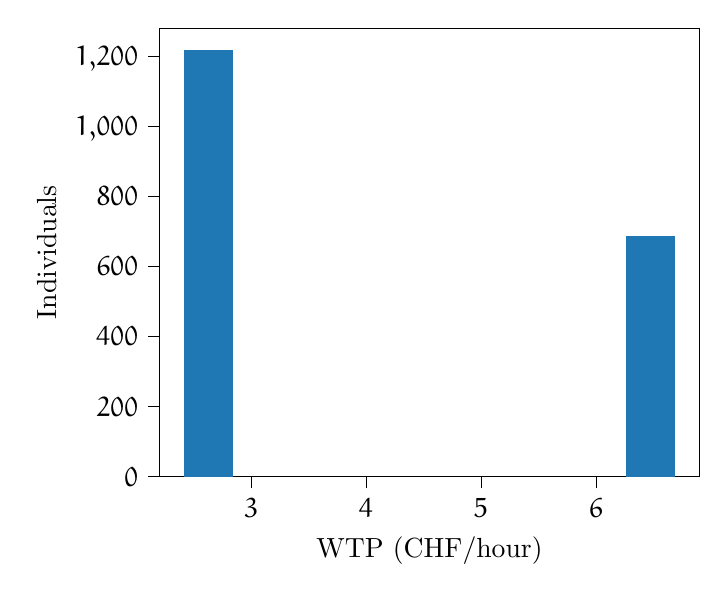
\begin{tikzpicture}

\definecolor{color0}{rgb}{0.12156862745098,0.466666666666667,0.705882352941177}

\begin{axis}[
tick align=outside,
tick pos=left,
x grid style={white!69.0196078431373!black},
xlabel={WTP (CHF/hour)},
xmin=2.20273789752521, xmax=6.90004114997706,
xtick style={color=black},
y grid style={white!69.0196078431373!black},
ylabel={Individuals},
ymin=0, ymax=1279.88244645484,
ytick style={color=black}
]
\draw[draw=none,fill=color0] (axis cs:2.41625168172757,0) rectangle (axis cs:2.84327925013228,1218.93566329032);
\draw[draw=none,fill=color0] (axis cs:2.84327925013228,0) rectangle (axis cs:3.270306818537,0);
\draw[draw=none,fill=color0] (axis cs:3.270306818537,0) rectangle (axis cs:3.69733438694171,0);
\draw[draw=none,fill=color0] (axis cs:3.69733438694171,0) rectangle (axis cs:4.12436195534642,0);
\draw[draw=none,fill=color0] (axis cs:4.12436195534642,0) rectangle (axis cs:4.55138952375114,0);
\draw[draw=none,fill=color0] (axis cs:4.55138952375114,0) rectangle (axis cs:4.97841709215585,0);
\draw[draw=none,fill=color0] (axis cs:4.97841709215585,0) rectangle (axis cs:5.40544466056056,0);
\draw[draw=none,fill=color0] (axis cs:5.40544466056056,0) rectangle (axis cs:5.83247222896528,0);
\draw[draw=none,fill=color0] (axis cs:5.83247222896528,0) rectangle (axis cs:6.25949979736999,0);
\draw[draw=none,fill=color0] (axis cs:6.25949979736999,0) rectangle (axis cs:6.68652736577471,687.064325016725);
\end{axis}

\end{tikzpicture}

\end{center}
\caption{\label{fig:wtp}Distribution of the willingness to pay in the sample}
\end{figure}
\section{Conclusion}

PandasBiogeme is a flexible tool that allows to extract useful
indicators from complex models. In this document, we have presented
how some indicators relevant for discrete choice models  can be
generated. As the output of the simulation is a Pandas data frame, a
great deal of analysis can be performed exploiting the functionalities of
Python, Pandas and Biogeme.


\clearpage

\appendix

\section{Mathematical expressions}\label{sec:expressions}

\renewcommand{\arraystretch}{1.2}
\subsection{Simple expressions}
Simple expressions can be calculated both with the functions
\lstinline@getValue@ (implemented in Python) and the \lstinline@getValue_c@ (implemented in C++). They do not require a database.
\begin{center}
\begin{tabular}{llll}
  &   Input  & Syntax & Output \\
  \hline
  Addition & $x$, $y$ & \lstinline@x + y@ & $x+y$ \\
  Substraction & $x$, $y$ & \lstinline@x - y@ & $x-y$ \\
  Multiplication & $x$, $y$ & \lstinline@x * y@ & $xy$ \\
  Division & $x$, $y$ & \lstinline@x / y@ & $\frac{x}{y}$ \\
  Power & $x$, $y$ & \lstinline@x ** y@ & $x^y$ \\
  Exponential & $x$ & \lstinline@exp(x)@ & $e^x$ \\
  Logarithm & $x$ & \lstinline@log(x)@ & $\ln(x) = \log_e(x)$ \\
  Minimum & $x$, $y$ & \lstinline@bioMin(x, y)@ & $\min(x, y)$ \\
  Maximum & $x$, $y$ & \lstinline@bioMax(x, y)@ & $\max(x, y)$ \\
  And & $x$, $y$ & \lstinline@x & y@ & 1 if $(x\neq 0)$ and $(y \neq 0)$ \\
      &          &                   & 0 otherwise \\
  Or & $x$, $y$ & \lstinline@x | y@ & 1 if $(x\neq 0)$ or $(y \neq 0)$ \\
      &          &                   & 0 otherwise \\
\end{tabular}
\end{center}
\begin{center}
\begin{tabular}{llll}
  &   Input  & Syntax & Output \\
  \hline
  Equal & $x$, $y$ & \lstinline@x == y@ & 1 if $x=y$ \\
      &          &                   & 0 otherwise \\
  Not equal & $x$, $y$ & \lstinline@x != y@ & 1 if $x\neq y$ \\
      &          &                   & 0 otherwise \\
  Lesser or equal & $x$, $y$ & \lstinline@x <= y@ & 1 if $x\leq y$ \\
      &          &                   & 0 otherwise \\
  Greater or equal & $x$, $y$ & \lstinline@x >= y@ & 1 if $x\geq y$ \\
      &          &                   & 0 otherwise \\
  Lesser & $x$, $y$ & \lstinline@x < y@ & 1 if $x < y$ \\
      &          &                   & 0 otherwise \\
  Greater & $x$, $y$ & \lstinline@x > y@ & 1 if $x > y$ \\
  &          &                   & 0 otherwise \\
  Opposite & $x$ & \lstinline@-x@ & $-x$ \\
  Multiple sum & $(x_i)_{i=1}^K$ &
  \lstinline@bioMultSum(listOfExpressions)@ & $\sum_{i=1}^K x_i$ \\
  Element &  $k, d = \{k: x_k\}_{k=1}^K$  & \lstinline@Elem(my_dict, index)@ & $d[k]$ \\
\end{tabular}
\end{center}

\subsection{Complex expression}

An expressions is deemed complex in Biogeme when the
\lstinline@getValue@ function is not available. Only the
\lstinline@getValue_c@ function must be used. It calculates the
expressions using a C++ implementation of the expression.

\renewcommand{\arraystretch}{2}

\begin{center}
\begin{tabular}{lllp{0.5\textwidth}}
  &   Input  & Syntax & Output \\
  \hline
  Normal CDF & $x$ & \lstinline@bioNormalCdf(x)@ &
  $\displaystyle\frac{1}{\sqrt{2\pi}}\int_{t=-\infty}^x e^{\frac{1}{2}t^2}dt$ \\
  Derivative & $x$ & \lstinline@Derive(x, 'y')@ & $\displaystyle\frac{\partial x}{\partial
    y}$ where $y$ is a literal expression. \\
  Integral & $f(\omega)$, $\omega$ & \lstinline@Integrate(f, 'omega')@ &
  $\displaystyle\int_{-\infty}^{+\infty} f(\omega) d\omega.$
\end{tabular}
\end{center}

  \subsection{Expression requiring a database}

\begin{center}
\begin{tabular}{p{0.15\textwidth}p{0.20\textwidth}p{0.35\textwidth}p{0.30\textwidth}}
  &   Input  & Syntax & Output \\
  \hline
  Linear utility & $(\beta_i, x_i)_{i=1}^K$ & \lstinline@bioLinearUtility(listOfTerms)@
  & $\displaystyle\sum_{i=1}^K \beta_i x_i$. \\
  Monte-Carlo & $x(\xi)$, $(\xi_r)_{r=1}^R$ &
  \lstinline@MonteCarlo(x)@ & $\displaystyle\frac{1}{R} \sum_{r=1}^R x(\xi_r)$\\
  Panel trajectory & $x$ & \lstinline@PanelLikelihoodTrajectory(x)@ &
  $\displaystyle\prod_{t=1}^{T_n} x_t$ \\
     &    &   & $x_1, \ldots x_T$ are expressions calculated on the
  $T$ entries associated with the same
  individual $n$ in panel data. \\
  \end{tabular}
\end{center}

\section{Complete specification files}

We provide here the code of the specification files used in this
document.

\subsection{\lstinline$01expression.py$}\label{sec:01expression}
\begin{lstlisting}[style=numbers]
import numpy as np
import matplotlib.pyplot as plt
from biogeme.expressions import Beta, exp


# We create a simple expression
b = Beta('b', 1, None, None, 0)
expression = exp(-b * b + 1)

# We can calculate its value.
z = expression.getValue_c()
print(f'exp(-b * b + 1) = {z}')

# We can also calculate the value, the first derivative, the second
# derivative, and the BHHH, which in this case is the square of the
# first derivatives

f, g, h, bhhh = expression.getValueAndDerivatives()
print(f'f = {f}')
print(f'g = {g}')
print(f'h = {h}')
print(f'BHHH = {bhhh}')

# From the expression, we can create a Python function that takes as
# argument the value of the free parameters, and returns the function,
# the first and second derivatives.
fct = expression.createFunction()

# We can use the function for different values of the parameter
beta = 2
f, g, h = fct(beta)
print(f'f({beta}) = {f}')
print(f'g({beta}) = {g}')
print(f'h({beta}) = {h}')

beta = 3
f, g, h = fct(beta)
print(f'f({beta}) = {f}')
print(f'g({beta}) = {g}')
print(f'h({beta}) = {h}')


# We can also use it to plot the function and its derivatives
x = np.arange(-2, 2, 0.01)
f = [fct(xx)[0] for xx in x]
g = [float(fct([xx])[1]) for xx in x]
h = [float(fct([xx])[2]) for xx in x]

ax = plt.gca()
ax.plot(x, f, label="f(x)")
ax.plot(x, g, label="f'(x)")
ax.plot(x, h, label='f"(x)')
ax.legend()
plt.show()
\end{lstlisting}

\subsection{\lstinline$scenarios.py$}\label{sec:scenarios}
\begin{lstlisting}[style=numbers]
import pandas as pd
import biogeme.database as db
from biogeme.expressions import Beta, Variable

# Read the data
df = pd.read_csv('optima.dat', sep='\t')
database = db.Database('optima', df)

# Variables from the data
Choice = Variable('Choice')
TimePT = Variable('TimePT')
TimeCar = Variable('TimeCar')
MarginalCostPT = Variable('MarginalCostPT')
CostCarCHF = Variable('CostCarCHF')
distance_km = Variable('distance_km')
Gender = Variable('Gender')
OccupStat = Variable('OccupStat')
Weight = Variable('Weight')

# Exclude observations such that the chosen alternative is -1
database.remove(Choice == -1.0)

# Normalize the weights
sumWeight = database.data['Weight'].sum()
numberOfRows = database.data.shape[0]
normalizedWeight = Weight * numberOfRows / sumWeight

# List of parameters to be estimated
ASC_CAR = Beta('ASC_CAR', 0, None, None, 0)
ASC_PT = Beta('ASC_PT', 0, None, None, 1)
ASC_SM = Beta('ASC_SM', 0, None, None, 0)
BETA_TIME_FULLTIME = Beta('BETA_TIME_FULLTIME', 0, None, None, 0)
BETA_TIME_OTHER = Beta('BETA_TIME_OTHER', 0, None, None, 0)
BETA_DIST_MALE = Beta('BETA_DIST_MALE', 0, None, None, 0)
BETA_DIST_FEMALE = Beta('BETA_DIST_FEMALE', 0, None, None, 0)
BETA_DIST_UNREPORTED = Beta(
    'BETA_DIST_UNREPORTED', 0, None, None, 0
)
BETA_COST = Beta('BETA_COST', 0, None, None, 0)

# Definition of variables:
# For numerical reasons, it is good practice to scale the data to
# that the values of the parameters are around 1.0.

TimePT_scaled = TimePT / 200
TimeCar_scaled = TimeCar / 200
CostCarCHF_scaled = CostCarCHF / 10
distance_km_scaled = distance_km / 5
male = Gender == 1
female = Gender == 2
unreportedGender = Gender == -1

fulltime = OccupStat == 1
notfulltime = OccupStat != 1


def scenario(factor=1.0):
    """Provide the model specification for a scenario with the price of
        public transportation is multiplied by a factor

    :param factor: factor that multiples the price of public transportation.
    :type factor: float

    :return: a dict with the utility functions, the nesting structure,
        and the choice expression.

    :rtype: dict(int: biogeme.expression), tuple(biogeme.expression,
        list(int)), biogeme.expression
    """
    MarginalCostScenario = MarginalCostPT * factor
    MarginalCostPT_scaled = MarginalCostScenario / 10
    # Definition of utility functions:
    V_PT = (
        ASC_PT
        + BETA_TIME_FULLTIME * TimePT_scaled * fulltime
        + BETA_TIME_OTHER * TimePT_scaled * notfulltime
        + BETA_COST * MarginalCostPT_scaled
    )
    V_CAR = (
        ASC_CAR
        + BETA_TIME_FULLTIME * TimeCar_scaled * fulltime
        + BETA_TIME_OTHER * TimeCar_scaled * notfulltime
        + BETA_COST * CostCarCHF_scaled
    )
    V_SM = (
        ASC_SM
        + BETA_DIST_MALE * distance_km_scaled * male
        + BETA_DIST_FEMALE * distance_km_scaled * female
        + BETA_DIST_UNREPORTED
        * distance_km_scaled
        * unreportedGender
    )

    # Associate utility functions with the numbering of alternatives
    V = {0: V_PT, 1: V_CAR, 2: V_SM}

    # Definition of the nests:
    # 1: nests parameter
    # 2: list of alternatives
    MU_NOCAR = Beta('MU_NOCAR', 1.0, 1.0, None, 0)

    CAR_NEST = 1.0, [1]
    NO_CAR_NEST = MU_NOCAR, [0, 2]
    nests = CAR_NEST, NO_CAR_NEST
    return V, nests, Choice, MarginalCostScenario
\end{lstlisting}

\subsection{\lstinline$01expressions.py$}\label{sec:01expressions}
\begin{lstlisting}[style=numbers]
import numpy as np
import matplotlib.pyplot as plt
from biogeme.expressions import Beta, exp


# We create a simple expression
b = Beta('b', 1, None, None, 0)
expression = exp(-b * b + 1)

# We can calculate its value.
z = expression.getValue_c()
print(f'exp(-b * b + 1) = {z}')

# We can also calculate the value, the first derivative, the second
# derivative, and the BHHH, which in this case is the square of the
# first derivatives

f, g, h, bhhh = expression.getValueAndDerivatives()
print(f'f = {f}')
print(f'g = {g}')
print(f'h = {h}')
print(f'BHHH = {bhhh}')

# From the expression, we can create a Python function that takes as
# argument the value of the free parameters, and returns the function,
# the first and second derivatives.
fct = expression.createFunction()

# We can use the function for different values of the parameter
beta = 2
f, g, h = fct(beta)
print(f'f({beta}) = {f}')
print(f'g({beta}) = {g}')
print(f'h({beta}) = {h}')

beta = 3
f, g, h = fct(beta)
print(f'f({beta}) = {f}')
print(f'g({beta}) = {g}')
print(f'h({beta}) = {h}')


# We can also use it to plot the function and its derivatives
x = np.arange(-2, 2, 0.01)
f = [fct(xx)[0] for xx in x]
g = [float(fct([xx])[1]) for xx in x]
h = [float(fct([xx])[2]) for xx in x]

ax = plt.gca()
ax.plot(x, f, label="f(x)")
ax.plot(x, g, label="f'(x)")
ax.plot(x, h, label='f"(x)')
ax.legend()

plt.show()
\end{lstlisting}

\subsection{\lstinline$02estimation.py$}\label{sec:02estimation}
\begin{lstlisting}[style=numbers]
from biogeme import models
import biogeme.biogeme as bio
from scenarios import scenario, database

# Obtain the specification for the default scenario
V, nests, Choice, _ = scenario()

# The choice model is a nested logit, with availability conditions
# For estimation, we need the log of the probability
logprob = models.lognested(V, None, nests, Choice)

# Create the Biogeme object for estimation
biogeme = bio.BIOGEME(database, logprob)
biogeme.modelName = '02estimation'

print('Estimation...')
# Estimate the parameters. Perform bootstrapping.
results = biogeme.estimate(bootstrap=100)

# Get the results in a pandas table
pandasResults = results.getEstimatedParameters()
print(pandasResults)

print('Simulation...')

simulated_choices = logprob.getValue_c(
    betas=results.getBetaValues(), database=database
)

print(simulated_choices)

loglikelihood = logprob.getValue_c(
    betas=results.getBetaValues(),
    database=database,
    aggregation=True,
)

print(f'Final log likelihood:     {results.data.logLike}')
print(f'Simulated log likelihood: {loglikelihood}')
\end{lstlisting}

\subsection{\lstinline$03simulation.py$}\label{sec:03simulation}
\begin{lstlisting}[style=numbers]
import sys
import time
import pandas as pd
from biogeme import models
import biogeme.biogeme as bio
import biogeme.exceptions as excep
import biogeme.results as res
from scenarios import scenario, database, normalizedWeight

# Obtain the specification for the default scenario
V, nests, _, _ = scenario()

V_PT = V[0]
V_CAR = V[1]
V_SM = V[2]

# Obtain the expression for the choice probability of each alternative
prob_PT = models.nested(V, None, nests, 0)
prob_CAR = models.nested(V, None, nests, 1)
prob_SM = models.nested(V, None, nests, 2)

# Read the estimation results from the file
try:
    results = res.bioResults(pickleFile='02estimation.pickle')
except excep.biogemeError:
    sys.exit(
        'Run first the script 02simulation.py '
        'in order to generate the '
        'file 02estimation.pickle.'
    )


# We now simulate various expressions on the database, and store the
# results in a Pandas dataframe

start_time = time.time()
simulate_formulas = {
    'weight': normalizedWeight.getValue_c(
        betas=results.getBetaValues(), database=database
    ),
    'Utility PT': V_PT.getValue_c(
        betas=results.getBetaValues(), database=database
    ),
    'Utility car': V_CAR.getValue_c(
        betas=results.getBetaValues(), database=database
    ),
    'Utility SM': V_SM.getValue_c(
        betas=results.getBetaValues(), database=database
    ),
    'Prob. PT': prob_PT.getValue_c(
        betas=results.getBetaValues(), database=database
    ),
    'Prob. car': prob_CAR.getValue_c(
        betas=results.getBetaValues(), database=database
    ),
    'Prob. SM': prob_SM.getValue_c(
        betas=results.getBetaValues(), database=database
    ),
}

simulated_values = pd.DataFrame.from_dict(
    simulate_formulas,
)
print(
    f'--- Execution time with getValue_c: '
    f'{time.time() - start_time:.2f} seconds ---'
)

# We now perform the same simulation using Biogeme. The results are be
# identical, but the execution time is faster. Indeed, Biogeme
# recycles calculations performed for one expression for the other
# expressions.

# A dictionary with the requested expression must be provided to Biogeme

simulate = {
    'weight': normalizedWeight,
    'Utility PT': V_PT,
    'Utility car': V_CAR,
    'Utility SM': V_SM,
    'Prob. PT': prob_PT,
    'Prob. car': prob_CAR,
    'Prob. SM': prob_SM,
}

start_time = time.time()
biogeme = bio.BIOGEME(database, simulate)
biogeme_simulation = biogeme.simulate(results.getBetaValues())
print(
    f'--- Execution time with Biogeme:    '
    f'{time.time() - start_time:.2f} seconds ---'
)

# Let's print the two results, to show that they are identical

print('Results without Biogeme')
print(simulated_values)
print('Results with Biogeme')
print(biogeme_simulation)
\end{lstlisting}

\subsection{\lstinline$04market_shares.py$}\label{sec:04market_shares}
\begin{lstlisting}[style=numbers]
import sys
from biogeme import models
import biogeme.biogeme as bio
import biogeme.exceptions as excep
import biogeme.results as res
from scenarios import scenario, database, normalizedWeight

# Obtain the specification for the default scenario
V, nests, _, _ = scenario()

# Obtain the expression for the choice probability of each alternative
prob_PT = models.nested(V, None, nests, 0)
prob_CAR = models.nested(V, None, nests, 1)
prob_SM = models.nested(V, None, nests, 2)

# Read the estimation results from the file
try:
    results = res.bioResults(pickleFile='02estimation.pickle')
except excep.biogemeError:
    sys.exit(
        'Run first the script 02simulation.py '
        'in order to generate the '
        'file 02estimation.pickle.'
    )

# We now simulate the choice probabilities and the weight

simulate = {
    'weight': normalizedWeight,
    'Prob. PT': prob_PT,
    'Prob. car': prob_CAR,
    'Prob. SM': prob_SM,
}

biogeme = bio.BIOGEME(database, simulate)
simulated_values = biogeme.simulate(results.getBetaValues())

# We also calculate confidence intervals for the calculated quantities

betas = biogeme.freeBetaNames
b = results.getBetasForSensitivityAnalysis(betas)
left, right = biogeme.confidenceIntervals(b, 0.9)


# Market shares are calculated using the weighted mean of the
# individual probabilities

# Alternative car
simulated_values['Weighted prob. car'] = (
    simulated_values['weight'] * simulated_values['Prob. car']
)
left['Weighted prob. car'] = left['weight'] * left['Prob. car']
right['Weighted prob. car'] = (
    right['weight'] * right['Prob. car']
)

marketShare_car = simulated_values['Weighted prob. car'].mean()
marketShare_car_left = left['Weighted prob. car'].mean()
marketShare_car_right = right['Weighted prob. car'].mean()

# Alternative public transportation
simulated_values['Weighted prob. PT'] = (
    simulated_values['weight'] * simulated_values['Prob. PT']
)
left['Weighted prob. PT'] = left['weight'] * left['Prob. PT']
right['Weighted prob. PT'] = right['weight'] * right['Prob. PT']

marketShare_PT = simulated_values['Weighted prob. PT'].mean()
marketShare_PT_left = left['Weighted prob. PT'].mean()
marketShare_PT_right = right['Weighted prob. PT'].mean()

# Alternative slow modes
simulated_values['Weighted prob. SM'] = (
    simulated_values['weight'] * simulated_values['Prob. SM']
)
left['Weighted prob. SM'] = left['weight'] * left['Prob. SM']
right['Weighted prob. SM'] = right['weight'] * right['Prob. SM']

marketShare_SM = simulated_values['Weighted prob. SM'].mean()
marketShare_SM_left = left['Weighted prob. SM'].mean()
marketShare_SM_right = right['Weighted prob. SM'].mean()

# Reporting
print(
    f'Market share for car: {100*marketShare_car:.1f}% '
    f'[{100*marketShare_car_left:.1f}%, '
    f'{100*marketShare_car_right:.1f}%]'
)
print(
    f'Market share for PT:  {100*marketShare_PT:.1f}% '
    f'[{100*marketShare_PT_left:.1f}%, '
    f'{100*marketShare_PT_right:.1f}%]'
)
print(
    f'Market share for SM:   {100*marketShare_SM:.1f}% '
    f'[{100*marketShare_SM_left:.1f}%, '
    f'{100*marketShare_SM_right:.1f}%]'
)
\end{lstlisting}

\subsection{\lstinline$05revenues.py$}\label{sec:05revenues}
\begin{lstlisting}[style=numbers]
import sys
import numpy as np
from tqdm import tqdm
from biogeme import models
import biogeme.exceptions as excep
import matplotlib.pyplot as plt
import biogeme.biogeme as bio
import biogeme.results as res
from scenarios import scenario, database, normalizedWeight

# Read the estimation results from the file
try:
    results = res.bioResults(pickleFile='02estimation.pickle')
except excep.biogemeError:
    sys.exit(
        'Run first the script 02simulation.py '
        'in order to generate the '
        'file 02estimation.pickle.'
    )


def revenues(factor):
    """Calculate the total revenues generated by public transportation,
        when the price is multiplied by a factor.

    :param factor: factor that multiplies the current cost of public
        transportation
    :type factor: float

    :return: total revenues, followed by the lower and upper bound of
        the confidence interval.
    :rtype: tuple(float, float, float)

    """
    # Obtain the specification for the default scenario
    V, nests, _, MarginalCostScenario = scenario(factor=factor)

    # Obtain the expression for the choice probability of each alternative
    prob_PT = models.nested(V, None, nests, 0)

    # We now simulate the choice probabilities,the weight and the
    # price variable

    simulate = {
        'weight': normalizedWeight,
        'Revenue public transportation': prob_PT
        * MarginalCostScenario,
    }

    biogeme = bio.BIOGEME(database, simulate)
    simulated_values = biogeme.simulate(results.getBetaValues())

    # We also calculate confidence intervals for the calculated quantities

    betas = biogeme.freeBetaNames
    b = results.getBetasForSensitivityAnalysis(betas)
    left, right = biogeme.confidenceIntervals(b, 0.9)

    revenues_pt = (
        simulated_values['Revenue public transportation']
        * simulated_values['weight']
    ).sum()
    revenues_pt_left = (
        left['Revenue public transportation'] * left['weight']
    ).sum()
    revenues_pt_right = (
        right['Revenue public transportation'] * right['weight']
    ).sum()
    return revenues_pt, revenues_pt_left, revenues_pt_right


# Current revenues for public transportation

r, r_left, r_right = revenues(factor=1.0)
print(
    f'Total revenues for public transportation (for the sample): {r:.1f} CHF '
    f'[{r_left:.1f} CHF, '
    f'{r_right:.1f} CHF]'
)

# We now investigate how the revenues vary with the multiplicative factor

factors = np.arange(0.0, 5.0, 0.05)

plot_revenues = [revenues(s) for s in tqdm(factors)]
zipped = zip(*plot_revenues)
rev = next(zipped)
lower = next(zipped)
upper = next(zipped)

largest_revenue = max(rev)
max_index = rev.index(largest_revenue)
print(
    f'Largest revenue: {largest_revenue:.1f} obtained with '
    f'factor {factors[max_index]:.1f}'
)

# We plot the results
ax = plt.gca()
ax.plot(factors, rev, label="Revenues")
ax.plot(factors, lower, label="Lower bound of the CI")
ax.plot(factors, upper, label="Upper bound of the CI")
ax.legend()

plt.show()
\end{lstlisting}

\subsection{\lstinline$06point_elasticities.py$}\label{sec:06point_elasticities}
\begin{lstlisting}[style=numbers]
import sys
import biogeme.biogeme as bio
from biogeme import models
import biogeme.results as res
import biogeme.exceptions as excep
from biogeme.expressions import Derive
from scenarios import (
    scenario,
    database,
    normalizedWeight,
    TimePT,
    TimeCar,
    MarginalCostPT,
    CostCarCHF,
    distance_km,
)


# Obtain the specification for the default scenario
V, nests, _, _ = scenario()

# Obtain the expression for the choice probability of each alternative
prob_PT = models.nested(V, None, nests, 0)
prob_CAR = models.nested(V, None, nests, 1)
prob_SM = models.nested(V, None, nests, 2)

# Calculation of the direct elasticities.
# We use the 'Derive' operator to calculate the derivatives.

direct_elas_pt_time = (
    Derive(prob_PT, 'TimePT') * TimePT / prob_PT
)

direct_elas_pt_cost = (
    Derive(prob_PT, 'MarginalCostPT') * MarginalCostPT / prob_PT
)

direct_elas_car_time = (
    Derive(prob_CAR, 'TimeCar') * TimeCar / prob_CAR
)

direct_elas_car_cost = (
    Derive(prob_CAR, 'CostCarCHF') * CostCarCHF / prob_CAR
)

direct_elas_sm_dist = (
    Derive(prob_SM, 'distance_km') * distance_km / prob_SM
)

# Simulate the formulas
simulate = {
    'weight': normalizedWeight,
    'Prob. car': prob_CAR,
    'Prob. public transportation': prob_PT,
    'Prob. slow modes': prob_SM,
    'direct_elas_pt_time': direct_elas_pt_time,
    'direct_elas_pt_cost': direct_elas_pt_cost,
    'direct_elas_car_time': direct_elas_car_time,
    'direct_elas_car_cost': direct_elas_car_cost,
    'direct_elas_sm_dist': direct_elas_sm_dist,
}

biogeme = bio.BIOGEME(database, simulate)

# Read the estimation results from the file
try:
    results = res.bioResults(pickleFile='02estimation.pickle')
except excep.biogemeError:
    sys.exit(
        'Run first the script 02estimation.py in order to generate '
        'the file 02estimation.pickle.'
    )

# simulatedValues is a Panda dataframe with the same number of rows as
# the database, and as many columns as formulas to simulate.
simulated_values = biogeme.simulate(results.getBetaValues())

# We calculate the aggregate elasticities

# First, the weighted probabilities
simulated_values['Weighted prob. car'] = (
    simulated_values['weight'] * simulated_values['Prob. car']
)
simulated_values['Weighted prob. PT'] = (
    simulated_values['weight']
    * simulated_values['Prob. public transportation']
)
simulated_values['Weighted prob. SM'] = (
    simulated_values['weight']
    * simulated_values['Prob. slow modes']
)

# Then the denominator of the aggregate elasticity expression.
denominator_car = simulated_values['Weighted prob. car'].sum()
denominator_pt = simulated_values['Weighted prob. PT'].sum()
denominator_sm = simulated_values['Weighted prob. SM'].sum()

# And finally the aggregate elasticities themselves.
direct_elas_term_car_time = (
    simulated_values['Weighted prob. car']
    * simulated_values['direct_elas_car_time']
    / denominator_car
).sum()
print(
    f'Aggregate direct point elasticity of car wrt time: '
    f'{direct_elas_term_car_time:.3g}'
)

direct_elas_term_car_cost = (
    simulated_values['Weighted prob. car']
    * simulated_values['direct_elas_car_cost']
    / denominator_car
).sum()
print(
    f'Aggregate direct point elasticity of car wrt cost: '
    f'{direct_elas_term_car_cost:.3g}'
)

direct_elas_term_pt_time = (
    simulated_values['Weighted prob. PT']
    * simulated_values['direct_elas_pt_time']
    / denominator_pt
).sum()
print(
    f'Aggregate direct point elasticity of PT wrt time: '
    f'{direct_elas_term_pt_time:.3g}'
)

direct_elas_term_pt_cost = (
    simulated_values['Weighted prob. PT']
    * simulated_values['direct_elas_pt_cost']
    / denominator_pt
).sum()
print(
    f'Aggregate direct point elasticity of PT wrt cost: '
    f'{direct_elas_term_pt_cost:.3g}'
)

direct_elas_term_sm_dist = (
    simulated_values['Weighted prob. SM']
    * simulated_values['direct_elas_sm_dist']
    / denominator_sm
).sum()
print(
    f'Aggregate direct point elasticity of SM wrt distance: '
    f'{direct_elas_term_sm_dist:.3g}'
)
\end{lstlisting}

\subsection{\lstinline$07cross_elasticities.py$}\label{sec:07cross_elasticities}
\begin{lstlisting}[style=numbers]
import sys
import biogeme.biogeme as bio
from biogeme import models
import biogeme.exceptions as excep
import biogeme.results as res
from biogeme.expressions import Derive
from scenarios import (
    scenario,
    database,
    normalizedWeight,
    TimePT,
    TimeCar,
    MarginalCostPT,
    CostCarCHF,
)


# Obtain the specification for the default scenario
V, nests, _, _ = scenario()

# Obtain the expression for the choice probability of each alternative
prob_PT = models.nested(V, None, nests, 0)
prob_CAR = models.nested(V, None, nests, 1)
prob_SM = models.nested(V, None, nests, 2)

# The choice model is a nested logit
prob_PT = models.nested(V, None, nests, 0)
prob_CAR = models.nested(V, None, nests, 1)
prob_SM = models.nested(V, None, nests, 2)

# Calculation of the cross elasticities.
# We use the 'Derive' operator to calculate the derivatives.
cross_elas_pt_time = (
    Derive(prob_PT, 'TimeCar') * TimeCar / prob_PT
)
cross_elas_pt_cost = (
    Derive(prob_PT, 'CostCarCHF') * CostCarCHF / prob_PT
)
cross_elas_car_time = (
    Derive(prob_CAR, 'TimePT') * TimePT / prob_CAR
)
cross_elas_car_cost = (
    Derive(prob_CAR, 'MarginalCostPT')
    * MarginalCostPT
    / prob_CAR
)

simulate = {
    'weight': normalizedWeight,
    'Prob. car': prob_CAR,
    'Prob. public transportation': prob_PT,
    'Prob. slow modes': prob_SM,
    'cross_elas_pt_time': cross_elas_pt_time,
    'cross_elas_pt_cost': cross_elas_pt_cost,
    'cross_elas_car_time': cross_elas_car_time,
    'cross_elas_car_cost': cross_elas_car_cost,
}

biogeme = bio.BIOGEME(database, simulate)

# Read the estimation results from the file
try:
    results = res.bioResults(pickleFile='02estimation.pickle')
except excep.biogemeError:
    sys.exit(
        'Run first the script 02estimation.py in order to generate '
        'the file 02estimation.pickle.'
    )

# simulated_values is a Panda dataframe with the same number of rows as
# the database, and as many columns as formulas to simulate.
simulated_values = biogeme.simulate(results.getBetaValues())

# We calculate the elasticities
simulated_values['Weighted prob. car'] = (
    simulated_values['weight'] * simulated_values['Prob. car']
)
simulated_values['Weighted prob. PT'] = (
    simulated_values['weight']
    * simulated_values['Prob. public transportation']
)

denominator_car = simulated_values['Weighted prob. car'].sum()
denominator_pt = simulated_values['Weighted prob. PT'].sum()

cross_elas_term_car_time = (
    simulated_values['Weighted prob. car']
    * simulated_values['cross_elas_car_time']
    / denominator_car
).sum()
print(
    f'Aggregate cross elasticity of car wrt time: '
    f'{cross_elas_term_car_time:.3g}'
)

cross_elas_term_car_cost = (
    simulated_values['Weighted prob. car']
    * simulated_values['cross_elas_car_cost']
    / denominator_car
).sum()
print(
    f'Aggregate cross elasticity of car wrt cost: '
    f'{cross_elas_term_car_cost:.3g}'
)

cross_elas_term_pt_time = (
    simulated_values['Weighted prob. PT']
    * simulated_values['cross_elas_pt_time']
    / denominator_pt
).sum()
print(
    f'Aggregate cross elasticity of PT wrt car time: '
    f'{cross_elas_term_pt_time:.3g}'
)

cross_elas_term_pt_cost = (
    simulated_values['Weighted prob. PT']
    * simulated_values['cross_elas_pt_cost']
    / denominator_pt
).sum()
print(
    f'Aggregate cross direct elasticity of PT wrt car cost: '
    f'{cross_elas_term_pt_cost:.3g}'
)

\end{lstlisting}

\subsection{\lstinline$08arc_elasticities.py$}\label{sec:08arc_elasticities}
\begin{lstlisting}[style=numbers]
import sys
import biogeme.biogeme as bio
import biogeme.exceptions as excep
from biogeme import models
import biogeme.results as res
from scenarios import (
    scenario,
    database,
    normalizedWeight,
)

# Obtain the specification for the default scenario
V, nests, _, MarginalCostPT = scenario()

# Obtain the expression for the choice probability of each alternative
prob_PT = models.nested(V, None, nests, 0)

# We investigate a scenario where the price for public transportation
# increases by 20%
V_after, _, _, MarginalCostPT_after = scenario(factor=1.2)
prob_PT_after = models.nested(V_after, None, nests, 0)


# Disaggregate elasticities
direct_elas_pt = (
    (prob_PT_after - prob_PT)
    * MarginalCostPT
    / (prob_PT * (MarginalCostPT_after - MarginalCostPT))
)

simulate = {
    'weight': normalizedWeight,
    'Prob. PT': prob_PT,
    'direct_elas_pt': direct_elas_pt,
}

biogeme = bio.BIOGEME(database, simulate)

# Read the estimation results from the file
try:
    results = res.bioResults(pickleFile='02estimation.pickle')
except excep.biogemeError:
    sys.exit(
        'Run first the script 02estimation.py in order to generate '
        'the file 02estimation.pickle.'
    )

# simulated_values is a Panda dataframe with the same number of rows as
# the database, and as many columns as formulas to simulate.
simulated_values = biogeme.simulate(results.getBetaValues())

# We calculate the elasticities
simulated_values['Weighted prob. PT'] = (
    simulated_values['weight'] * simulated_values['Prob. PT']
)

denominator_pt = simulated_values['Weighted prob. PT'].sum()

direct_elas_pt = (
    simulated_values['Weighted prob. PT']
    * simulated_values['direct_elas_pt']
    / denominator_pt
).sum()

print(
    f'Aggregate direct arc elasticity of public transportation wrt cost: '
    f'{direct_elas_pt:.3g}'
)
\end{lstlisting}

\subsection{\lstinline$09wtp.py$}\label{sec:09wtp}
\begin{lstlisting}[style=numbers]
import sys
import matplotlib.pyplot as plt
import biogeme.biogeme as bio
import biogeme.exceptions as excep
import biogeme.results as res

from biogeme.expressions import Derive
from scenarios import (
    scenario,
    database,
    normalizedWeight,
)

V, _, _, _ = scenario()

V_PT = V[0]
V_CAR = V[1]

WTP_PT_TIME = Derive(V_PT, 'TimePT') / Derive(
    V_PT, 'MarginalCostPT'
)
WTP_CAR_TIME = Derive(V_CAR, 'TimeCar') / Derive(
    V_CAR, 'CostCarCHF'
)

simulate = {
    'weight': normalizedWeight,
    'WTP PT time': WTP_PT_TIME,
    'WTP CAR time': WTP_CAR_TIME,
}

biogeme = bio.BIOGEME(database, simulate)

# Read the estimation results from the file.
try:
    results = res.bioResults(pickleFile='02estimation.pickle')
except excep.biogemeError:
    sys.exit(
        'Run first the script 02estimation.py in order to generate '
        'the file 02estimation.pickle.'
    )

# simulated_values is a Panda dataframe with the same number of rows as
# the database, and as many columns as formulas to simulate.
simulated_values = biogeme.simulate(results.getBetaValues())

wtpcar = (
    60
    * simulated_values['WTP CAR time']
    * simulated_values['weight']
).mean()

# Calculate confidence intervals
b = results.getBetasForSensitivityAnalysis(biogeme.freeBetaNames)

# Returns data frame containing, for each simulated value, the left
# and right bounds of the confidence interval calculated by simulation.
left, right = biogeme.confidenceIntervals(b, 0.9)

wtpcar_left = (60 * left['WTP CAR time'] * left['weight']).mean()
wtpcar_right = (
    60 * right['WTP CAR time'] * right['weight']
).mean()
print(
    f'Average WTP for car: {wtpcar:.3g} '
    f'CI:[{wtpcar_left:.3g}, {wtpcar_right:.3g}]'
)


# In this specific case, there are only two distinct values in the
# population: for workers and non workers
print(
    'Unique values:      ',
    [
        f'{i:.3g}'
        for i in 60 * simulated_values['WTP CAR time'].unique()
    ],
)


def wtpForSubgroup(theFilter):
    """
    Check the value for groups of the population. Define a function that
    works for any filter to avoid repeating code.

    :param theFilter: pandas filter
    :type theFilter: numpy.Series(bool)

    :return: willingness-to-pay for car and confidence interval
    :rtype: tuple(float, float, float)
    """
    size = theFilter.sum()
    sim = simulated_values[theFilter]
    totalWeight = sim['weight'].sum()
    weight = sim['weight'] * size / totalWeight
    _wtpcar = (60 * sim['WTP CAR time'] * weight).mean()
    _wtpcar_left = (
        60 * left[theFilter]['WTP CAR time'] * weight
    ).mean()
    _wtpcar_right = (
        60 * right[theFilter]['WTP CAR time'] * weight
    ).mean()
    return _wtpcar, _wtpcar_left, _wtpcar_right


# full time workers.
aFilter = database.data['OccupStat'] == 1
w, l, r = wtpForSubgroup(aFilter)
print(f'WTP car for workers: {w:.3g} CI:[{l:.3g}, {r:.3g}]')

# females
aFilter = database.data['Gender'] == 2
w, l, r = wtpForSubgroup(aFilter)
print(f'WTP car for females: {w:.3g} CI:[{l:.3g}, {r:.3g}]')

# males
aFilter = database.data['Gender'] == 1
w, l, r = wtpForSubgroup(aFilter)
print(f'WTP car for males  : {w:.3g} CI:[{l:.3g}, {r:.3g}]')

# We plot the distribution of WTP in the population. In this case,
# there are only two values

plt.hist(
    60 * simulated_values['WTP CAR time'],
    weights=simulated_values['weight'],
)
plt.xlabel('WTP (CHF/hour)')
plt.ylabel('Individuals')
plt.show()
\end{lstlisting}



\clearpage

\bibliographystyle{dcu}
\bibliography{../dca}

\end{document}
